% The sequence of commands that you need to run. 
% Note: We are using the xindy option of the glossaries package. That must be installed as well as Perl. 
% 
% pdflatex Dissertation
% pdflatex Dissertation
% makeglossaries Dissertation
% pdflatex Dissertation
% bibtex Dissertation
% pdflatex Dissertation
%
% Alternatively you can just run the custom script by typing sh compileAll.sh

\documentclass[dissertation,CC-BY-ND]{uathesis}

\usepackage[a4paper,width=150mm,top=25mm,bottom=25mm]{geometry}
\usepackage[T1]{fontenc}
\usepackage[utf8]{inputenc}
\usepackage{authblk}
\usepackage{graphicx}
%\usepackage{natbib}
%\usepackage{chapterbib}
\usepackage[cmex10]{amsmath}
\usepackage{amssymb}
\usepackage{amsthm}
\usepackage{mathrsfs}
\usepackage{hyphenat}
\usepackage{url}
\usepackage[bookmarks,colorlinks=true,urlcolor=black,linkcolor=black,citecolor=black]{hyperref}
\usepackage{cleveref}
\usepackage[utf8]{inputenc}

% This package allows us to make a list of acronyms, the option nomain is used
% because we actually don't want a glossary, the second option is used because 
% we want to define acronyms and display a list of used acronyms, 
\usepackage[nomain,acronyms,xindy]{glossaries}

% This is rquires to make a glossary, a list of acronyms, or a list of 
\makeglossaries
\glstoctrue

%%%%%%%%%%%%%%%%%%%%%%%%%%% Define acronyms here% %%%%%%%%%%%%%%%%%%%%%%%%%%%%%

\newacronym{svm}{SVM}{support vector machine}
\newacronym[plural=FPAs,firstplural=focal-plane arrays (FPAs)]{fpa}{FPA}{focal-plane array}
\newacronym{psf}{PSF}{point spread function}
\newacronym{adc}{ADC}{analog-to-digital converter}
\newacronym{afssi-c}{AFSSI-C}{Adaptive Feature Specific Spectral Imaging-Classifier}
\newacronym{pca}{PCA}{Principal Component Analysis}
\newacronym{LENS}{LENS}{Laboratory for Engineering Non-Traditional Sensors}
\newacronym{scout}{SCOUT}{Static Computational Optical Undersampled Tracker}
\newacronym{disp}{DISP}{Duke Imaging and Spectroscopy Program}
\newacronym{lcos}{LCOS}{Liquid Crystal on Silicon}
\newacronym{slm}{SLM}{Spatial Light Modulator}
\newacronym{snr}{SNR}{Signal-To-Noise Ratio}
\newacronym{swap-c}{SWAP-C}{Size, Weight and Power-Cost}

%%%%%%%%%%%%%%%%%%% End of acryonym defintions here %%%%%%%%%%%%%%%%%%%%%%%%%%%%%

\crefname{section}{Section}{Sections}
\crefname{figure}{Figure}{Figures}
\crefname{table}{Table}{Tables}
\setcounter{secnumdepth}{3} 
\setcounter{tocdepth}{3}

\include{newcommands}

\completetitle{Practical Considerations in Experimental Computational Sensing}
\fullname{Phillip K. Poon}			% Grad college wants your full name here.
\degreename{Doctor of Philosophy}	% Title of your degree.

\begin{document}
\maketitlepage
{COLLEGE OF OPTICAL SCIENCES} % Title of the department
{2016}	

\approval
{12 December 2016}		% Defense Date	
{Amit Ashok}  		% 1st committee member
{Rongguang Liang}		% 2nd committee membe
{Michael E. Gehm}

\statementbyauthor
% If this is a Thesis, use the following form, with your thesis director's
% name and title in the square brackets like so (you should also omit the 
% approval form insertion above):
%\statementbyauthor[Jane M. Doe\\Professor of Chemistry]

% Include the ``Acknowledgements''
\incacknowledgements{acknowledgements}

% Include the ``Dedication''
\incdedication{dedication}

% Create a ``Table of Contents''
\tableofcontents

% Create a ``List of Figures''
\listoffigures
% Create a ``List of Tables''
\listoftables

% Include the ``Abstract''
\incabstract{abstract}

%\printglossary[type=htypei]

\chapter{Introduction}\label{chap:Introduction}


This chapter introduces the reader to the concepts of \gls{isomorphic sensing}, \gls{multiplex sensing}, \gls{indirect-imaging}, \gls{task-specific sensing}, \gls{compressive sensing} and \gls{computational sensing}. It also provides the motivation for the need to address the practical issues in experimental computational sensing. 

A \gls{measurement} is a process that converts a physical phenomena to a collection of data. The signal-of-interest is the physical phenomena that we are interested in quantifying. We will call the collection of data the measurement data. Often the measurement is \emph{\gls{isomorphic}}. \Gls{isomorphic sensing} is the concept that a sensor's measurement data resembles the signal-of-interest. \Gls{isomorphic sensing} is called \gls{traditional sensing}. In isomorphic sensing the analog hardware, \acrfull{adc}, and processing algorithms are all seperate components, see Figure \ref{fig:isomorphicsesingflowchart}. \Gls{computational sensing} is the concept that a joint design of the sensor, often though \emph{coding} of the analog signal, with inversion algorithms can exceed the performance of an isomorphic sensor. \Glspl{computational sensor} exist at the intersection of these processes, see Figure \ref{fig:computationalsensingflowchart} \cite{neifeld2006taskSpecificSensing}. While \gls{isomorphic} sensors can provide flexible sensing in multiple applications, a \gls{computational sensor}'s joint design can lead to performance increases. Throughout this chapter and the rest of this dissertation, we will provide many examples that highlight the differences between computational and isomorphic sensing. 

\begin{figure}
    \centering
    \includegraphics[scale=1]{isomorphicsensorflowchart}
    \caption{A systems view of a traditional sensing scheme. The signal-of-interest is incident upon the analog instrument. The analog instrument forms an isomorphism of the signal which is then periodically sampled point-by-point through an \gls{adc} device. Once the signal is in digital form, post-processing algorithms are often used to perform various tasks such as noise reduction, detection, and classification. Notice that the analog instrument, sampling scheme, and processing are all seperated. }
    \label{fig:isomorphicsesingflowchart}
\end{figure}


\begin{figure}
    \centering
    \includegraphics[scale=1]{computationalsensingflowchart}
    \caption{A systems view of a computational sensing scheme. The signal-of-interest is incident upon the analog instrument.  }
    \label{fig:computationalsensingflowchart}
\end{figure}


Rather than a rigorous discussion, this chapter will discuss some of the major developments and concepts in the field of computational sensing on an intuitive level. This will familiarize the reader with important terminology and techniques common in the field of computational sensing. A rigorous discussion with mathematical formalism of the concepts is presented in \autoref{chap:Formalism}. This chapter will also discuss some of the challenges I and many other experimentalists and engineers have faced when developing computational sensing prototypes. I will close this chapter with a brief look ahead to the rest of the dissertation. 

%History%%%%%%%%%%%%%%%%%%%%

\section{Isomorphic Sensing}\label{sec:Isomorphic Sensing}

In Greek, the word isomorphic loosely translates to equal in form. Traditional sensors perform isomorphic sensing. In the context of this dissertation, an isomorphic sensor is any sensor which attempts to produces measurement data that resembles the signal-of-interest. In this paradigm, the analog instrument, sampling scheme, and post-processing algorithms are seperate components and processes.

We will discuss three important examples of isomorphic sensors: the pinhole camera, the photographic camera and the optical spectrometer (which I will just call a spectrometer from now on, even though there are many instruments called spectromers that not concerned with optical spectra). These sensors have had major roles throughout the history of optics and in the physical sciences, so it is natural to use them as examples of computational optical sensing. Therefore it is important we first understand the isomorphic version of these sensors.

In the photographic camera, the signal-of-interest is the object's intensity distribution. This can be the scatter or emitted light from a person, a tree or a distant group of stars. The analog instrument consists of the lenses which are designed and fabricated to produce an intensity disibution (optical image) that looks like the object at the \gls{fpa}. The more that the image resembles the object the better the optics. The \gls{fpa} then samples and quantizes the image and produces a digital representation of the object's intensity distribution, the measurement data. If one is interested in performing a task such as detection or classification, the measurement data is often is post-processed to perform those tasks. 


There are two major sub-systems in the photographic camera which determine how well it performs: the optics and the FPA. Ideally, the optics (the analog instrument in this case) will produce a \gls{psf} which is infinitely small in diameter. For example, in a task such as the detection of a star from several neighboring stars in the night sky, if the \gls{psf} is much larger than the center to center seperation of the two stars in the optical image, it will be quite difficult to detect. A careful reader will note that this is the same argument used by Lord Raleigh in proposing his resolution criterion \cite{rayleigh1879investigations}. Even if the \gls{psf} is small enough, the \gls{fpa} must sample at a fine enough pixel-to-pixel spacing, called the \gls{pixel pitch}, to accurately reproduce the intensity variations at the scale which is pertinant to the task. Intuitively, this makes sense because if the image of the stars are imaged onto a single pixel, then one cannot ever hope to be able to accurately the detect the star without some other prior or side information. 

The pinhole camera consists of a small hole and a box which prevents any light except from the pinhole to enter, see Figure \ref{fig:pinholecamera}. The pinhole camera is useful for imaging in parts of the electromagnetic spectrum and particles for which there is no direct analog to refractive lens or reflective mirror. Like the photographic camera, the pinhole camera also attempts to produce a small \gls{psf} for better spatial resolution and a human observer, film, or \gls{fpa} can be used to measure the object scene. As the hole size decreases, the spatial resolution increase at the cost of reducing the signal strength.

\begin{figure}
    \centering
    \includegraphics[scale=1]{pinholecamera}
    \caption{A pinhole camera.}
    \label{fig:pinholecamera}
\end{figure}

In the spectrometer, the signal of interest is the spectrum of the object. The optics are designed to take the incoming light and seperate various wavelength components, see Figure \ref{fig:slitspectrometer}. The part of the spectrometer which is used to physically isolate the wavelengths is called a \gls{monochromator}. The result is a spectral intensity as a function of position at the \gls{fpa}. The \gls{fpa} and post-processing algorithms are used in the same manner as the photographic camera, which is to sample the optical spectrum creating a digital version of it and to perform various tasks on the measurement data. For now, we will concentrate on the slit spectrometer, which measures the spectrum at a single point on the object.


\begin{figure}
    \centering
    \includegraphics[scale=1]{slitspectrometer}
    \caption{An isomorphic slit spectrometer with a 4F configuration.}
    \label{fig:slitspectrometer}
\end{figure}

In the spectrometer, one of the important performance metrics is \gls{spectral resolution}, which we denote \gls{specres}. The spectral resolution is the smallest difference in wavelength the instrument can discern. Large spectral resolutions can degrade the spectrometers ability to discern important parts of the spectrum. Similarly with the camera, the \gls{fpa} must have a \gls{pixel pitch} which is small enough in order to correctly sample the variations in the spectrum. 

The point-by-point nature of isomorphic sensing is both a strength and a source of weakness. 

The strength comes from the straightforward and intuitive architecture of the isomorphic sensor. Each subsystem: the optics, the \acrfull{fpa}, and the post-processing can be designed and constructed seperately as long as they meet their individual specifications. As long as the \gls{snr} is sufficient and the sampling rate is high enough, we are guaranteed to recover the signal.

One of the weaknessess of the isomorphic approach is the the ability to measure low \gls{snr} signals. Because the signal-of-interest is sampled in a completely parallel fashion at each exposure, each pixel contributes a certain amount of noise. If the noise dominates, the measurement fidelity decreases often forcing the operator to increase the exposure time. For weak signals, the exposure time can become prohibitive and for temporally dynamic signals this may lead to a loss of resolution. Indeed, one of the major engineering trade-offs faced by traditional spectrometer designers is that when one attempts to increase the light collection (increased slit-width) the spectral resolution \gls{specres} degrades. Similarly, in the pinhole camera, there is a throughput versus spatial resolution trade-off, increasing the size of the pinhole degrades the \gls{psf}.

It would be easy to assume that with the recent revolution in machine learning and statistical signal processing combined with the dramatic increase in computing power that we could simply post-process poor measurments and obtain useful data. However, this isn't possible due to the an important theorem in information theory called the \gls{data processing inequality} \cite{cover2012elements}. In layman's terms, it means "garbage in, garbage out".

Another weakness of isomorhic sensing is that the seperation of the analog instrument, the sampling scheme, and the data processing algorithms lead to increased \gls{swap-c}. As we mentioned in the photographic camera, the optics must be designed to produce a small \gls{psf}. For demanding applications, the optical design and fabrication can be the most expensive component of the sensor. While \gls{fpa} prices in the visible have fallen, \glspl{fpa} in certain parts of the electromagnetic spectrum can be quite expensive or non-existant \cite{watts2014terahertz, noor2011compressive}.

In many cases, the signal is redundant and high resolution sampling becomes a waste of resources, such as data storage and communications bandwidth. A good example is in photography where often the post-processing takes the digital image and applies a compression algorithm which looks for patterns in the signal and reduces the file size, discarding much of the sample data \cite{taubman2012jpeg2000}. 

The isomorphic sensor has served humanity well, however with all the weakness that I have discussed, I will now begin to discuss some of major techniques in computational sensing that can be used to address some or all of the issues that I just stated. 

\section{Development of Multiplexing in Sensing}\label{sec:multiplexInSensing}

\Gls{multiplexing} in sensing allows each measurement sample to be a combination of multiple points of the signal-of-interest.  Multiplexing is a powerful tool that can be exploited by the sensor designer to eliminate or relax design trade-offs. 

A simple example which illustrates the usefulness of multiplex sensing is weighing objects. In this example, we are given a 100 sheets of paper. Let's assume that the scale's measurement error is insignificant. Isomorphic measurement sensing means one would need to measure each sheet of paper individually. Requiring 100 measurements. 

Now, let's say the scale's measurement error is on the order of the weight of the sheet. Measuring each sheet invidiually produces a large measurement error. In order to reduce the error to an acceptable \gls{snr} we need to make several measurements per sheet to reduce the error to an acceptable level.

However, we can be a little smarter. We can measure all 100 sheets at the same time. Since the weight of all 100 sheets is much larger than the measurement error of the scale, we can dramatically increase the precision of the measurement. If we can assume that each sheet is the same weight, then we are done. 

The weighing problem is analogous to the spectroscopy example. As discussed earlier in \autoref{sec:Isomorphic Sensing}, there is trade-off between light collection and spectral resolution. Increasing the slit-width to increase the amount of light has the effect of degrading the spectral resolution \gls{specres}. Around the late 1940's and early 1950's, several important papers and inventions demonstrated the effectiveness of multiplexing in spectroscopy. At the time the \gls{fpa} was non-existant, so in the slit spectrometer shown in Figure \ref{fig:slitspectrometer}, where the \gls{fpa} is pictured, there was actually another slit. To record the intensity at each spectral channel, either the dispersive element or the exit slit had to be mechanically translated, making the measurements even slower by a factor of \gls{numspecchan}, the number of spectral channels of interest. 

Golay was the first to propose multiplexing the slit spectrometer by creating a pattern of binary (1's and 0's) entrance and exit slits \cite{golay1949multi}. The idea borrowed heavily from communications theory which is concerned with the reliable transmission of information over a noisey channel. In the Golay multi-slit spectrometer, the patterns of entrance and exit slits are matched based on mathematically useful properties, this is similar to coding and decoding signals in commucations. In communications theory the process of structuring the data from the source to the receiver is referred to as \gls{coding}. Similarly, in computational sensing, the transmission of information between a object signal-of-interest and the sensor is considered a coding problem \cite{brady2009optical}. In the multi-slit spectrometer, the entrance slits act to code the spectrum while the exit slits decoded the coded spectrum. Intuitively, the ability to use multiple entrance and exit slits increases the optical throughput of the spectrometer. Golay's idea dramatically increased the optical throughput without degrading the spectral resolution. 

Another example that is pertinant to this dissertation is coded aperture imaging. Coded aperture imaging can be thought of as the multiplexed version of a pinhole camera. As mentioned earlier in \autoref{sec:Isomorphic Sensing}, there is a trade-off between the throughput and spatial resolution. However in many fields, such as high-energy particle imaging, refractive lenses and reflective mirrors are non-existant or underdeveloped. By using multiple pinholes the throughput is increased without sacraficing spatial resolution. However, the pattern of the pinholes, which is the code, in this case must be carefully designed in order to the reconstruction to be feasible. Fenimore, Canon, and Gottesman were the first to create an elegant solution to coded aperture design called uniformly redundant arrays \cite{fenimore1978coded, gottesman1989new}.

In summary, multiplexing has the ability to eliminate classic trade-offs in isomoprhic sensors: signal strength or resolution. Modern researchers are still actively developing novel ways to implement multiplexing to increase resolution and senstivity in the spatial domain \cite{duarte2008single, townsend2012static}, spectral domain \cite{gehm2006static, tsai2013coded}, and temporal domain \cite{holloway2012flutter,llull2013coded}. However, multiplexing is not without its own set of challenges. As we mentioned, the coding must often be designed to obtain feasible signal reconstruction. We now discuss inverse problems in computational sensing.

\section{Forward Models and Inverse Problems}

In the computational sensing community, a model explains the mapping of the signal-of-interest to the measurement data is called the \gls{forward model}. The problem of taking the observed data and calculating a reconstruction of the signal-of-interst or task-specific parameters is called the \gls{inverse problem}.

As you can imagine, solving inverse problems of isomorphic measurements, when one is concerned with reconstruction of the signal-of-interest, tend to be straight forward. In the weighing problem, the measurement is also the reconstruction. In the slit spectromer, where the forward model can be simply the continuous to discrete mapping of the spectrum. The spectrum is the interpolated measurement. 

Of course, we can begin to add various levels of complexity to the forward model to account for various physical aspects of the sensor, such as the fact the \gls{fpa} can't measure certain wavelength regions or the noise in our measurements. But again, assuming proper sampling and enough \gls{snr}, the reconstruction of the isomorphic signal is the measurement. This simplicity is one reason why isomorphic sensing still dominates at the consumer level despite all of the drawbacks I discussed earlier in \autoref{sec:Isomorphic Sensing}. 

However, the multiplexing of signal information forces us to develop computational steps to solving the inverse problem. In the multiplexed weighing problem, a significant complication occurs when each sheet of paper has a different weight. Now solving the inverse problem is not as straight forward. A single measurement of all 100 sheets in this case is an underdetermined problem, since we have 1 equation and 100 unknowns. What we can do is try measuring different combinations of the 100 sheets, each new combination provides us with a new equation to work with reducing the error. Niavely, we might assume that we can randomly choose 100 unique combinations and solve 100 equations using the algebra we were taught in high school. This works fine when there is no measurement error. However, in the presense of noise, in many applications including the weighing problem, random combinations are not the best way to conduct the coding. They are sub-optimal in terms of reconstruction error. This lead many to begin working on optimal coding strategies of signals for sensing and is major topic in this disseration.

In fact, the idea of multiplexing was not invented by Golay or Fenimore, what they contibuted was the creation of effective ways to code and decode their signal-of-interest, making their sensors more appealling to a broader community of scientists and engineers.

In summary, the forward model of a sensor is essentially accounting for the physics which govern the measurement. While the solving the inverse problem is a mathematical problem which attempts to either reconstruct the object or to calculate task-specific data from the measurement data. Unfortunately, not all multiplexing forward models codes have mathematically elegent inversion steps. Often the physics of the situation force non-isomorphic measurements which require a computational step to solve the inverse problem. 

\section{Indirect Imaging}

While Golay, Fennimore, and others were levering multiplexing to eliminate trade-offs in traditional sensors, an entirely disparate group of researchers were working on imaging techniques for which there was no isomorphic analog. In these cases the physics of the sensing modality prevents a point-by-point sampling of the signal-of-interest. Indirect imaging refer to sensing schemes which include X-ray \gls{ct}, \gls{spect}, \gls{pet}, \gls{mri} and certain forms of sonic and radio wave imaging all require a data-processing or reconstruction step to solve an inverse problem \cite{barrett2013foundations}. 

Perhaps one of the most successful early examples of indirect imaging and the rise of inverse problems in sensing is the development of radar. While early radar was concerned with the detection and distance of an object, development of imaging radar began after World War II. Imaging radar and specifically \gls{sar} can use time delay information combined with the doppler effects and interference patterns of coherent radio waves to create high resolutions of terrain and buildings. 

In medicine, a common imaging modality is X-Ray \gls{ct}. In X-Ray \gls{ct}, computational inversion is required to reconstruct a 2 or 3-dimensional function from 1 or 2-dimensional measurement data. The forward model can be simple: In a collimated beam architecture with a 1-dimensional detector array, we say that each sample from each pixel on the array is proportional to the total number of x-ray photons that have not been absorped by the object \cite{radon20051} plus noise. The inversion of course is not straight forward. The culmination of the work related to the inversion techniques and the actual prototype resulted in the Nobel Prize for Physiology or Medicine in 1979 \cite{nobelprize1979medicine}. 

Indirect imaging is a subfield of computational sensing. Due to the medical or military applications of these computational sensors, there has been an intense push to reduce measurement time and improve task-specific and reconstruction results. Many of the techniques from other subfields of computational sensing have been brought to bear for indirect imaging \cite{zhu2010tomographic, chen2012compressive}. 

We have discussed the development of multiplex sensing and indirect imaging and how the ideas from both subfields are analogous in terms of producing a non-isomorphic measurement. However a major step in practical implementation of computational sensing is being able to obtain the measurements in a quick, reliable and efficient manner. Computational sensing as a field would not exist without the most important invention in optics and photonics of the 20th century. 

\section{The Digital Imaging Revolution}

In 1969 Boyle and Smith invented the \gls{ccd} \cite{boyle1970charge}. The \gls{ccd} is the first integrated circuit device which using a 2-dimensional arrangement of pixels which could reliably convert an intensity distribution to a digital signal. The \gls{ccd} is a type of \gls{fpa}. 

The \gls{ccd} was a major breakthrough for entire fields and industries who depended on the reliable sampling, storage and transmission of optical signals. Until then one either had to use film or bulky tubes that required an electron beam to be scanned across an image scene, such as the Image orthicon \cite{w1975image}. For their invention, Boyle and Smith both received the Nobel Prize in Physics in 2009 \cite{nobelprize2009physics}

The invention of the digital camera by Sasson followed shortly after \cite{kodaksfirstdigital2015}. Several years later the first digital spectrometer was invented. The exit slit was replacing by the \gls{ccd}, whiched allowed for instant and simultaenous measurement of the entire spectrum in a compact architecture \cite{moore1979spectrometer}. 

The development of the \gls{cmos} \gls{fpa} was also important. While in scientific settings, it could not rival the quality of the \gls{ccd}, its cheaper cost brought digital imaging to the consumer level. Other technology like the digital computers and computer networking also provided major contributions to the democratization of imaging and optical sensing. While scientific grade optical instrumentation was and is still expensive, the researcher could at least capture, process, and share measurement data with significantly less effort. Without it, the field of computational sensing would not exist.

Algorithms for efficient and reliable storage and transmission of digital images became more important. Over time the pixel count continued to increase and the sheer volume of digtal image and video data being generated and transmitted over networks began to outpaced improvements in storage and transmission capacity. While many engineers developed new technology to combat the hardware limitations of storage and transmission. This also led to a renewed effort by researchers to develop more efficient image and video compression algorithms \cite{kobayashi1974image, ziv1978compression}. 

While a multitude of compression techniques exist, they all follow the same basic process, see Figure \ref{fig:imagecompressionflowchart}. Once the \gls{ccd} samples the optical signal and produes the measurement data, the encoder usings the compression algorithm to look for redundancies in the data and produce a lower dimensional representation of the image. The compressed data can then either be stored or transmitted or both. The decoder solves the inverse problem of reconstructing the image. 

\begin{figure}
    \centering
    \includegraphics[scale=1]{imagecompressionflowchart}
    \caption{An general flowchart for image and data compression techniques.}
    \label{fig:imagecompressionflowchart}
\end{figure}

As mentioned in at the beginning of this chapter, computational sensing lies at the intersection of the design of the analog hardware, sampling schemes, and processing algorithms. Many of the algorithms used in computational sensing are the same as or inspired by the techniques used by the image processing community. This is because a major effort of computational sensing is the desire to make more resource efficient measurements. 

\section{Compressive Sensing}\label{sec:multiplexingtocompressivesensing}

Traditionally, in order to increase the resolution of a sensor, one had to increase the number of measurements. This means that the \gls{swap-c} must also increase. A camera with just a few megapixels \gls{fpa} costs less than one with hundreds of megapixels. The cost of designing the optics will also need to scale to provide enough optical resolution. In a perfect world, we could capture all the information we need from just a few measurements.

Conventional signal processing dictates that accurate reconstruction of the signal-of-interest is highly improbable. If we have a discrete signal we need at least as many measurements as there are signal elements to solve the inverse problem. If the number of measurements is less, then the inverse problem is underdeterimined. Fortunately, a signal acquisition technique called \gls{compressive sensing} allows us to design sensors that solve these types of highly underdetermined inverse problems.

As discussed earlier, much of the data being generated by sensors are redundant. Images, spectra, video, and audio data of real-world signals tend to exhibit patterns or redundancies that can be exploited. This allows a compression algorithm to significantly reduce the amount of data needed to represent the signal. 

There is a class of compression algorithms called lossy \cite{usevitch2001tutorial}. In lossy compression, not only are redundancies exploited but data that is deemed insignificant to the signal quality is discarded. Only the most important part of the signal is kept as part of the compressed representation of the original signal. When the signal is uncompressed, the amount of data is less that the original measured data. The difference in quality is often unnoticeable to a human observer. In both lossless and lossy compression, the goal is to obtain a \gls{sparse} representation of the signal. A sparse representation means that the signal can be well approximated with only a few non-zero elements in a representation basis. A representation basis is a basis in which the signal-of-interest is sparse. For example, most natural images are sparse in the Fourier basis. The representation basis is typically not the native basis of the signal-of-interest, i.e. pixel number or spectral channel.

In 2006, David Donoho argued that traditional sensors tend to produce vast amounts of measurement data, but often the majority of data is redundant and discarded in the compression step. He proposed that sensors can be designed to directly measure the most relavent data in a signal, suggesting a measurement scheme that can measure a compressed form of the signal \cite{donoho2006compressed}. This is the idea behind \gls{compressive sensing} sometimes known as \gls{compressive sampling}. If the measurements are compressive then it should be possible to significantly reduce the number of measurements to accurately reconstruct the signal. 

Note that there is a subtle but powerful distinction between compressive sensing and the traditional approach of sensing and then compressing. In the traditional approach, compression algorithms operate as a post-processing step. Therefore, a traditional compression algorithm will have access to the entire signal to look for redundancies and convert it into a sparse representation. In compressive sensing, we attempt the compression directly and therefore do not have access to the entire uncompressed signal. The algorithms must assume that the signal has a sparse representation. 

The question of how to actually measure or code the analog signal to directly obtain compressed data is also important. Fortunately, random coding tends to work well in many instances when the signal has a sparse representation. Much of the work in this dissertation will discuss other types of coding schemes that can be used to outperform random codes. 

The idea of compressive sensing seems to be similar to the concept of multiplex sensing. However, there is an important distinction to be made. In compressive sensing, the aim is to obtain the relavent information in as few measurements as possible. In multiplexing, the goal is to overcome limitations mainly due to lack of \gls{snr}. Many compressive sensing schemes also employ multiplexing.

One useful example of compressive sensing versus traditional sensing is the single pixel camera \cite{duarte2008single}. The single pixel camera is a multiplexing camera architecture that uses time sequential random measurements and recovers the image in significantly less measurements (=number of exposures $\times$ pixels) than the conventional camera, see Figure \ref{fig:singlepixelcamera}. Another example is the \gls{cassi} architecture \cite{wagadarikar2008single}, which can reconstruct a spectral data cube in significantly less \gls{fpa} exposures than a traditional spectral imaging architecture. 


\begin{figure}
    \centering
    \includegraphics[scale=1]{singlepixelcamera}
    \caption{A single pixel camera architecture.}
    \label{fig:singlepixelcamera}
\end{figure}

Another important distinction is between reconstruction and task-specific sensing. Task-specific sensing tends to refer to measurement techniques that attempt to directly perform tasks such as detection, classification, and estimation without the intermiediate step of reconstructing the high-dimensional signal. Compressive sensing is useful not just of overcoming resolution limitations in reconstruction but for reducing measurement resources for task-specific sensing. For example, in facial recognition the goal is detection of an individual person. Reconstruction of the face image is simply an intermediate step, therefore, one can develop a compressive sensing scheme that is optimal for direct facial detection, skipping the step of image reconstruction \cite{pal2005face}. 

Multiplex sensing, compressive sensing, and task-specific sensing are considered subfields of computational sensing. Computational sensors offer significant advantages that allow us to overcome classic engineering trade-offs in sensor design. However, computational sensing has its own unique set of engineering problems that we will now discuss.

\section{Practical Considerations in Computational Sensing}

So far we have the discussed the development of computational sensing techniques and how they are used to ameliorate trade-offs in traditional sensor design. Computational sensing as a field is continuing to grow at a rapid pace. The number of journal publications related to computational sensings has steadily increases every year since 2008 \cite{stern2016hurdles}. There is now a major OSA meeting dedicated to computational sensing called \gls{cosi} \cite{cosi2016meetingwebsite} and textbooks dedicated to its study and development \cite{brady2009optical, foucart2013mathematical}. It is important to recognize is that while it is a powerful approach to radically new sensor architectures, challenges remain in our ability to design and demonstrate experimental practical computational sensors.

One of the major obstables in computational sensing is calibration. Calibration is the act of quanitying the sensor's measurements in order to produce an accurate forward model. While many traditional sensors also require calibration, computational sensors tend to be more sensitive to calibration error. 

There are two main reasons for this. The first reason is simply due to the fact that non-isomorphic measurements require a computational step to solve an inverse problem. The algorithms rely on accurate knowledge of the forward model to seperate measurement data due to the instrument and data due to the signal-of-interest. 

The second reason is due to the lack of redundancy in a compressive sensor's measurement. The redundancies that are typically deemed wasteful in traditional sensing, can also be used by post-processing algorithms to solve the inverse problem in a robust fashion. If the calibration is wrong for a few measurement sames, one can still use error-correcting algorithms to recover the comprimised data. In a compressive measurement, these redunancies are exploited in the physical measurement process \cite{gehm2013calibration}. Only a few numbers are used to repesent many. If the few numbers are misinterrepted due to poor calibration, the inversion algorithm's performance will suffer. We will illustrate in this dissertation the calibration challenges in several computational sensors. 

Since, calibration has become a major drawback in \gls{compressive sensors}. A consumer cannot be expected to spend time calibrating everytime the instrument is physically bumped or the air pressure changes. In high dimensional compressive sensors like hyperspectral imagers, the calibration time can last hours.

Another hurdle in the implementation of practical computational sensing is the need for prior knowledge. For example, in compressive imaging we have to assume the signal is sparse in some basis. Fortunately most realistic objects are sprase or compressible with modern representation bases, such as the wavelet basis. However, sometimes one needs to image something that is difficult to represent with any current basis, such as the intensity pattern due to laser speckle. One needs an alternative representation basis, so training sets are often used to generate a new basis in which the signal can be represented as sparse. One must generate many different example training data so a particular signal-of-interest can be have a sparse representation in that basis. This becomes time and compuationally expensive. Many algorithms require some prior knowledge of the statistics of the signal and noise ahead of time for optimal performance. A good example of this is the \gls{afssi-c}, a computational spectral classifier which requires knowledge of standard deviation of the noise's probability density function to perform spectral classification in the least number of measurements as possible.

Reducing the number of detector elements is often the goal in computational sensing. A notable example is the single pixel camera is an architecture. However, the single pixel camera requires several time sequential measurements. Each measurement displays a different \gls{dmd} pattern to create a randomly encoded measurements \cite{duarte2008single}. The drawback to this architecture is that one must point the camera at the object scene until enough measurements have been collected for proper reconstruction. A complication arises when this architecture is used to image temporally varying object scenes. One must display the \gls{dmd} patterns even faster and reduce the exposure time to keep up. As a result the \gls{snr} may begin to degrade. 

A possible way to mitigate this issue is to do all the encoding in parallel. However, a completely parallel approach would require a lens, a \gls{dmd} (or coded aperture), and a detector pixel for each measurement. Since each lens uses a different entrance pupil, this will means that each will have a slightly different view of the object scene. This drastically scales the complexity of the architecture and algorithms. In this dissertation, I will discuss a compromise to parallel coding, in two different computational sensors, by using a common entrance pupil and a \gls{ccd}.

Much of the Often, theorectically optimal measurements take advantage of codes which are simultaneously positive and negative. In reality, with incoherent light we are unable to make negative measurements. One is often forced into situations where one must record two sets of measurements and subtract one set of measurements from the positive set of measurements. This means an additional noise term is added to each effective measurement. 

Algorithms engineered to solve the inverse problems often do not account for the non-negativity of many physical situations. For example, in spectral unmixing where the problem is to solve for concentration of each material's spectrum. A non-negative fractional abundance that sums to one is a physical requirement. However, there is a serious lack of sparsity promitting algorithms that are able to enforce both the non-negativity and the sum to one constraint. 

A major issue in both the theoretical and experimental compressive sensing community is a lack of code design schemes. For the most part random measurements techniques are dominant because they obey a key theorectical result which guarantees reconstruction with high probability. Intuitively, designed, meaning non-random, measurement codes which can take into account prior knowledge of the physical limitations of the sensing task and statistical assumptions of the signal-of-interest should be able to outperform random measurements. For example, we will show that in certain applications we can use \gls{pca} to outperform random measurements. In one application, we will demonstrate that simply designed codes outperform random codes in low \gls{snr} environments. However, as of yet there is no adaptive measurement package one can simply take  ``out-of-the-box'' and begin applying them to compuational sensing problems and outperform random measurements on a consistent basis.

These issues and others will be discussed in a case study manner throughout this dissertation. I will now discuss the organization of this dissertation and the three seperate computational sensors I have built and how I have tried to migitate and resolve some of the practical issues associated with computational sensing.

\section{Dissertation Overview}

I used this chapter to cover the major concepts of computational sensing. More importantly, I provided the major topic of discussion for this dissertation, the challenges that are remain towards developing practical computational sensors. I will use the next chapter as an opportunity to provide a more detailed and mathematically rigorous look at the various coding schemes that are popular in computational sensing, as well as the ones I have used. This includes a discussion of the mathematical methods that I and my collaborators developed and deployed in the \gls{afssi-c}: Bayes rule, Log-Likelihood Ratios, and the Maximum a Posteriori decision technique. A more rigourous treatment of compressive sensing will also be provided which includes several important results from the compressive sensing community. I will also talk about several optimization algorithms and estimation techniques that have been used during the development of the three computational sensors in my work.

\Cref{chap:Scout} will introduce a new system architecture for compressive target tracking---the Static Computational Optical Undersampled Tracker (SCOUT). This system is designed to overcome a variety of challenges that typically arise in traditional optical sensing approaches. It provides several advantages over the single-pixel camera architecture, notably it can capture many simultaneous encodings of the field-of-view with a single camera exposure. I will present experimental results that validate the performance of the proposed architecture. 

\Cref{chap:Afssic} will discuss an important experimental protoype which demonstrates adaptive spectral image classification. The system is a major experimental advancement compared to current computational spectral imaging architectures which focus on reconstruction. Furthermore, the ability to perform adaptive measurements, where each code is designed based on the history of prior measurement data allows this instrument to outperform traditional spectral imaging architectures by a factor of 100 in low \gls{snr} scenarios.

\Cref{chap:Csu} will discuss current efforts to experimentally demonstrate compressive spectral unmixing. Often in spectral imaging, the spectra present in the field-of-view of each pixel is actual a mixture of several spectra, a mixed spectrum. Spectral unmixing is the task of inferring the fraction of each constituent spectrum in the mixed spectrum. I employ a unique architecture for computational spectral sensing which uses no diffraction grating or refracting prism but relies on the wavelength dependent nature of the birefringence in an \gls{lcos}. We will demonstrate the effectiveness of various compressive sensing measurement schemes to outperform a traditional sensor in significantly less measurements. 

\Cref{chap:Conclusion} will summarize the dissertation and provide my perspective on how the field should the approach the issues in practical computational optical sensing.


%\bibliographystyle{IEEEtranS}  
%\bibliography{ThesisBib}


\chapter{Formalism}\label{chap:Formalism}

This chapter introduces the reader to the more rigorous concepts and mathematical background that will required to fully understand the material presented in the later chapters of this dissertation. 

A rigorous discussion of multiplexing and signal-to-noise ratio will be discussed, as well are various coding schemes used in various notable computational sensors as well as the ones in this disseration. 

Since the \gls{afssi-c} relies on a variation of Principal Component Analysis (PCA) and a Bayesian algorithm for coding design we will discuss some of the fundamental of Bayesian probability and the Log-Likelihood Ratios. 



\section{Multiplexing}

\section{Principal Component Analysis}

\section{Bayesian Rules and Log-Likelihood Ratios}

\section{Compressive Sensing}

\subsection{The Nyquist-Shannon Sampling Theorem}

The Nyquist-Shannon Sampling Theorem states one must sample a signal with a sampling rate that is at least twice the maximum frequency of the signal to prevent aliasing \cite{shannon1949communication}.


\subsection{Sparsity, Incoherence, and the Restricted Isometry Property}

\subsection{Inversion}

\subsubsection{L0 and L1 Norm Minimization}

\subsubsection{LASSO and sparsity regularization}

%\bibliographystyle{IEEEtranS}  
%\bibliography{ThesisBib}




%\chapter{Static Computational Optical Undersampled Tracker}\label{chap:Scout}

\section{Motivation for the Static Computational Undersampled Tracker}

In large-area persistent surveillance, traditional \gls{isomorphic} sensing systems must acquire, process, store, and transmit large amounts of data to achieve high spatial and temporal resolution. These sensors are typically on airborne platforms or orbiting satellites which leads to a large \acrfull{swap-c}. However, if one is interested in estimating the location of moving objects (tracking) rather than reconstructing the entire object scene, the information content in the signal-of-interest is relatively low. One can significantly lower the \gls{swap-c} by using a task-specific approach. To address the challenges of traditional target tracking, several colleagues and I designed, built, and demonstrated such a device called the \acrfull{scout} \cite{townsend2012static, stenner2010static}. This chapter will provide details in to how we developed the \gls{scout}.

Most of the current experimental demonstrations of \gls{compressive imaging} try to reconstruct the entire object scene or spatial-temporal datacube. For example, the \gls{cacti} sensor uses a temporally varying psuedo-random coded aperture during a single \gls{fpa} exposure and attempts to reconstruct a spatial-temporal datacube \cite{llull2013coded}. In another experimental compressive imager, a rotating cylindrical lens measures scene data using an optical Radon transform and then reconstructs a static object scene \cite{evladov2012progressive}. While these architectures demonstrate the rapid progress that researchers have made towards compressive imaging, they emphasize reconstructing high dimensional data and require another post-processing step to extract task-specific information. Furthermore, this data will then need to be compressed again for storage or transmission. If one is concerned with only tasks, then reconstructing the entire scene as an intermediate step is unnecessary and even wasteful. 

Another example of \gls{compressive imaging} is the single pixel camera, discussed in \Cref{sec:multiplexingtocompressivesensing}. This sensor uses a \acrfull{dmd} to measure in any arbitrary basis, but must do so over many time-sequential measurements \cite{duarte2008single}. Each measurement is an integrated point-by-point multiplication of the scene locations with the \gls{dmd} array values. For temporally static scenes, this architecture allows an arbitrarily long exposure time (within the limit of detector saturation) to increase the \gls{snr} for each measurement. However, with temporally varying scenes it needs to record all the projections for each frame before the object moves.  Increasing the rate at which projections are made is possible, but this reduces exposure time and \gls{snr}. One way to overcome this is by implementing a parallel architecture of single pixel cameras, each with a different projection, see \Cref{fig:parallelcsimager2}. Clearly this will significantly increase the \gls{swap-c} of the architecture. Another issue with a fully parallel architecture, is that each camera will have a different entrance pupil location, producing parallax. One issue many computational sensor designs must deal with is ``over multiplexing''. All real optical \gls{adc} devices have a certain amount of dynamic range, in which linearity is valid. As the amount of light that is recorded increases, the amount of dynamic range being used fills up. Architectures which only use a single pixel are at greater risk for over multiplexing. 

\begin{figure}
	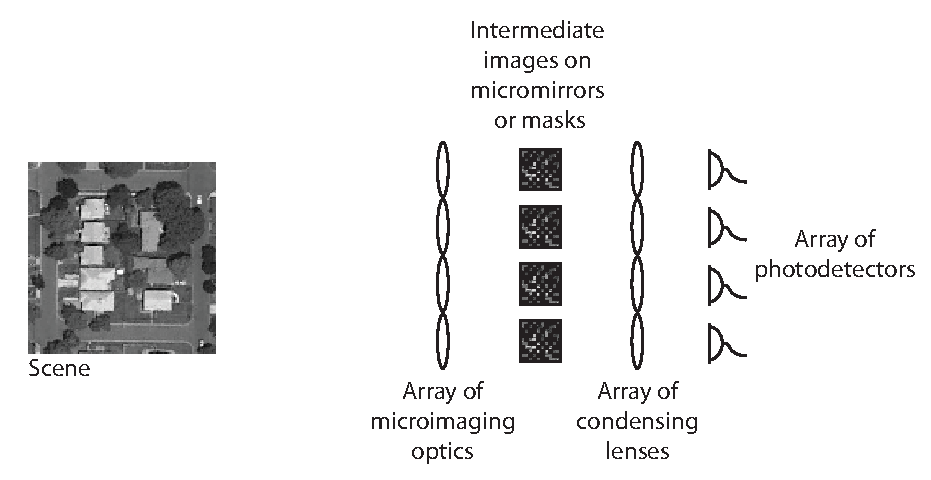
\includegraphics[scale=0.9]{parallelcsimager2}
	\captionof{figure}[The architecture of a hypothetical parallel single pixel camera to capture simultaneous projections.]{An example of a typical parallel optical CS architecture. Capturing $N_m$ simultaneous projections requires using $N_m$ spatial light modulators or masks and $N_m$ detector elements.}
	\label{fig:parallelcsimager2}
\end{figure}

A computational sensing architecture dedicated to target tracking rather than full object scene reconstruction, can significantly ameliorate these design trade-offs. We developed the \acrfull{scout} with the goal that measurements must be acquired ``single-shot'' using a conventional \gls{fpa} \cite{townsend2012static, poon2012advances}. The \gls{scout} system is an important step toward practical low-cost computational sensing for optical imaging. The system enables parallel ``single-shot'' acquisition of compressed, task-specific sensing oriented data, using a static (no moving parts) architecture. 

\begin{figure}
	\centering
	\includegraphics[scale=1.0]{scoutFlowchart}
	\captionof{figure}[Flowchart of \gls{scout} system architecture.]{A systems level flowchart of the \gls{scout} system. Light from the object scene propagates to the optical instrument which consists of a coded aperture (mask 1), an objective lens, and another coded aperture (mask 2), a \acrfull{fpa} then undersamples the coded object scene, measurement data is used to solve a \gls{lasso} problem. The parameters of the optical instrument is optimized using simulations to minimize the probability of tracking error. Calibration provides accurate measurement of the system matrix $\mb{H}$ to lasso optimization algorithm.}
	\label{fig:scoutFlowChart}
\end{figure}

A related static approach uses optical Radon projections \cite{kashter2012optical}. This instrument relies on a several cylindrical lenses to integrate the optical intensity from the object plane onto lines on the \gls{fpa}. The number of detector elements is much less than the native dimensionality of the object scene. For a single moving point in the field-of-view, two perpendicular Radon projections is enough to compute the change from frame to frame. However, the researchers found heuristically that four cylindrical lens are better for reconstructing the change information for an scene that included up to ten moving objects, called movers. 

A systems level flowchart of the \gls{scout} is shown in \Cref{fig:scoutFlowChart}. Like many computational sensors, it relies on the coding of the analog signal-of-interest prior to the \gls{adc} step and processes the measurement data using prior information and calibration data. The analog instrument was optimized using a custom ray-based simulation which evaluates a metric based on the simulated system matrix. In this chapter, I will discuss the \gls{scout} architecture in detail in \Cref{sec:ScoutArchitecture}, which uses a defocused imaging system with two binary amplitude masks. The \gls{fpa} samples at a much lower resolution than the native resolution of the object scene. While other compressive imaging systems have to reconstruct entire images, the \gls{scout} only reconstructs frame-to-frame differences. As a result the \gls{scout} requires significantly less bandwidth to transmit to a base station where the post-processing step can occur.


\section{SCOUT Architecture}\label{sec:ScoutArchitecture}

The goal of the \gls{scout} was to demonstrate a low \gls{swap-c} compressive target tracking sensor. The \gls{scout} architecture is designed to avoid the hardware scaling issues of the single-pixel camera. The trade-off for the ability to measure parallel projections is the loss of flexibility to implement arbitrary projections i.e. by using a \gls{slm}. However, rather than fully designing the projections themselves, I describe a process for optimizing the optical instrument  in \Cref{sec:ScoutSimulations}. Previous prototypes of the \gls{scout} architecture are described in \cite{stenner2010static, rivenson2010single}. 

The \gls{scout} system takes measurements that are both compressive and multiplexed: The number of measurements is less than the number of scene locations $N_m \ll N$, and each measurement must contain information about many scene locations. In this architecture, the number of measurements is the number of pixels in the \gls{fpa}. Intuitively this means that the system matrix must exhibit a many-to-few mapping from scene locations to \gls{fpa} elements. 


The \gls{scout} architecture is shown in \Cref{fig:scoutArchitecture}. In this architecture the \gls{multiplexing} occurs in the spatial domain by mapping multiple object scene locations to only a few detector pixels. To accomplish this, we created a structured blur. This blur allows the light from a single object point to be spread to several pixels on the \gls{fpa}. The most straightforward way to achieve a blur is by defocusing the image so that the \gls{psf} is broad, spanning many \gls{fpa} pixels. Since the number of \gls{fpa} pixels are less than the object scene resolution, the measurement is compressive. 


Like any aberration, defocus significantly reduces contrast of high spatial frequencies, so the measurements will be poorly conditioned for reconstruction. Therefore, we created high-frequency structure in the \gls{psf} by using two pseudo-random binary occlusion masks. Each mask is placed at different positions between the lens and the sensor. The separation between masks results in a spatially varying point-spread function. 




\begin{figure}
	\includegraphics[scale=1.2]{scoutArchitecture}
	\captionof{figure}[The SCOUT architecture.]{A diagram of the \gls{scout} architecture. A lens projects light through a pair of binary occlusion masks onto a low-resolution sensor which is defocused from the nominal image plane. This creates a spatially multiplexed shift-variant PSF incident on the \gls{fpa}.  }
	\label{fig:scoutArchitecture}
\end{figure}



As with many linear computational sensing architectures, the forward model is written in the form
%
\begin{equation}
	\mb{g} = \mb{H} \mb{f} + \mb{e}
\end{equation}
%
where $\mb{f}$ is the discrete representation of the object signal-of-interest, $\mb{g}$ is the measurement, $\mb{H}$ is the matrix which describes mapping of the object to the measurement, and $\mb{e}$ is the noise at each measurement. In this situation the signal-of-interest is actually the difference between two subsequent object scenes (frames) $\Delta \mb{f}$:
%
%
\begin{equation} 
\begin{split}
	\mb{g}_{k} &= \mb{H} \mb{f}_{k} + \mb{e}_{k} \\
	\mb{g}_{k+1} &= \mb{H} \mb{f}_{k+1} + \mb{e}_{k+1}
\end{split}
\end{equation}
%
Where the subscripts represent the $k^{th}$ readout from the \gls{fpa}.
%
\begin{equation}
	\Delta \mb{g} = \mb{g}_{k+1} - \mb{g}_{k} = \mb{H} \ap{ \mb{f}_{k+1} - \mb{f}_{k} } + \mb{e}_{k+1} - \mb{e}_{k} 
\end{equation}
%
%
so the forward model can be written as
%
\begin{equation}
	\Delta \mb{g} = \mb{H} \Delta \mb{f}  + \Delta \mb{e}
	\label{eq:scoutgHf}
\end{equation}
%
In this equation, the 2-dimensional difference frame and object scene have a resolution of $ R_x \times R_y$ elements, and are lexicography reordered into a $N \times 1$ column vector, $\Delta \mb{f}$ and $\mb{f}$. Similarly, the difference measurement and measurement $\Delta \mb{g}$ and $\mb{g}$ are $N_m \times 1$ vectors representing a 2-dimensional \gls{fpa} readout with a $ r_x \times r_y$ matrix which represents the low resolution measurement. The detector noise is represented by the $ N_m \times 1 $ vector $\mb{e}$. The system matrix $\mb{H}$ is thus an $N_m \times N $ matrix, where $N_m \ll N$ in order to the system to be considered compressive. The $n^{th}$ column of the matrix is the \gls{psf} of the $n^{th}$ location in the object scene. The resulting system matrix $\mb{H}$ demonstrates that the \gls{scout} is a spatially variant optical system and presents a block structure, as seen in the example shown in \Cref{fig:scoutSysResponse}.

\begin{sidewaysfigure}
	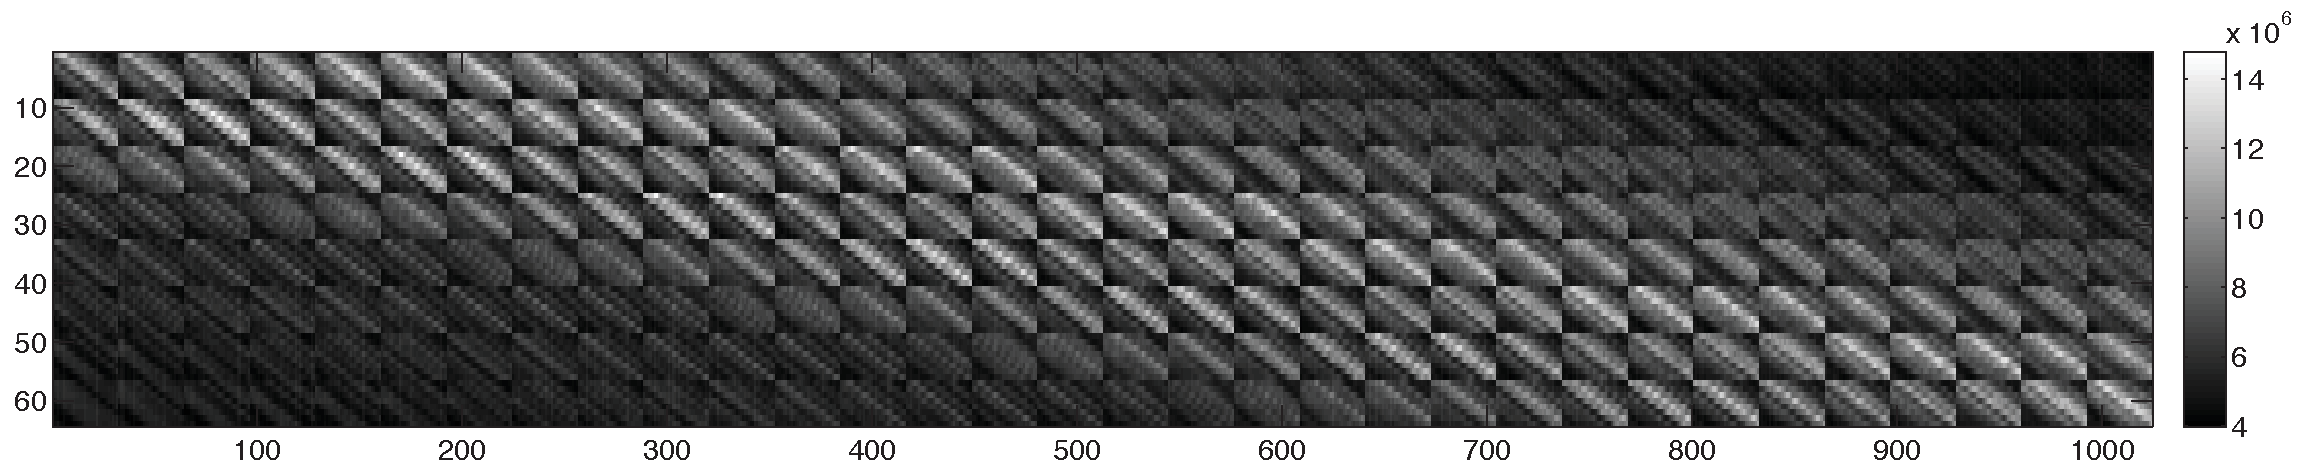
\includegraphics[scale=0.65]{scoutSysResponse}
	\captionof{figure}[An example of the system matrix of the \gls{scout}.]{An example of an experimentally measured of the system matrix of the \gls{scout} system. The approximate block-Toeplitz structure is clearly evident, as is the deviation from the Bernoulli or Gaussian ensembles typically considered in CS treatments. }
	\label{fig:scoutSysResponse}
\end{sidewaysfigure}


Referring back to the diagram of the \gls{scout} architecture shown in \Cref{fig:scoutArchitecture}. The object distance is much larger than the focal length of the lens so image of the scene occurs approximately one focal length from the lens $f_E$. The \gls{fpa} is placed some distance $d_{im}$ from the focal plane thus the total distance from the lens to the \gls{fpa} is $f_E + d_{im}$. Two binary occlusion masks, mask 1 and mask 2, are placed at distances $d_1$ and $d_2$ from the sensor. Mask 1 and 2 have associated fill factors $F_1$ and $F_2$ and pitch $p_1$ and $p_2$, respectively. 


\section{Optimizing the SCOUT}\label{sec:ScoutSimulations}

While the \gls{scout} lacks the ability to implement arbitrary measurement codes, we are able to adjust various physical parameters of the system such as defocus distance and mask fill factor to minimize reconstruction error. Adjusting each parameter in the actual prototype requires too much time, a more practical approach is to simulate the \gls{scout} architecture. In this section, I will discuss the simulation and define a metric that we used to evaluate different design parameters of the \gls{scout} without the need to reconstruct the difference frames. 

\subsection{Simulating a SCOUT System}

We developed a paraxial ray based simulation for the \gls{scout}. The simulation allows us to model the effects on the measurement as light travels through the lens and two masks and onto the detector plane. The lens is modeled as a single thin lens with transmittance function $t_f$ and the two masks have transmittance functions $t_1$ and $t_2$. From calibration measurements, the mask has a transmittances of $0$ where the mask is black and $0.88$ where the mask is clear. The lateral magnification of the scene and the two masks is calculated using similar triangles.

A simulated calibration occurs, in other words the simulation records the $r_x \times r_y$ PSF from each scene location in order to obtain the system matrix $\mb{H}$. Once $\mb{H}$ is known, we use it to simulate the low resolution measurements, $\mb{g}$, of the higher resolution scenes, $\mb{f}$. Subsequent simulated measurements are subtracted to find $\Delta \mb{g}$. We also did not add any noise. I have attached the simulation code in Appendix \ref{app:scoutSimCode}.


\subsection{Quantifying Reconstruction Error}

The \gls{mse} error metric is not suitable for our application because it weights all errors equally. For the task of motion tracking we classify errors into three types. A false positive occurs when the estimate shows an object where there is none. A false negative occurs when the estimate fails to show an object where one exists. As shift error occurs when an object is being tracked but appears in the wrong location. We developed a custom tracking error metric that weighs false negatives and false positives more than shift errors. This is because false negatives and false positives indicate a serious failure in the motion tracking task, while shift errors are less serious. We define tracking error as

\begin{equation}
	P = \frac{ | \mb{a}   \otimes \mb{\epsilon} |}{2N_{mv}}
	\label{eq:scoutErrorMetric}
\end{equation}
%
where
%
\begin{equation}
	\mb{a} = 
	\begin{bmatrix}
	    1/9 & 1/9 & 1/9 \\
	    1/9 & 1/9 & 1/9 \\
	    1/9 & 1/9 & 1/9 
	\end{bmatrix}
\end{equation}
%
where the error $\mb{\epsilon}$ is the difference between the true and reconstructed difference frames
%

\begin{equation}
	\mb{\epsilon} = \Delta \mb{f} - \Delta \mbh{f}
\end{equation}
%
and $N_{\text{mv}}$ is the number of movers in the scene. To reduce the penalty for one-pixel shift errors, the error frame is convolved with a three pixel averaging kernel $\mb{a}$. The absolute value is taken in order to count positive and negative errors equally, and the error is divided by $2N_{mv}$ to make the metric independent of the number of movers. 

\subsection{Optimizing Optical System Parameters}

Now that I have explained the simulation and the custom error metric for tracking, I can finally begin to discuss how we optimized some of the parameters to reduce the reconstruction error. Both the simulation and experimental study demonstrates a relationship between mask position and pitch: the tracking error is very sensitive to the \emph{projected} mask pitch on the \gls{fpa}. Furthermore, increasing the mask seperation reduced tracking error, generating a highly space-variant \gls{psf}. With these observations in mind, we focus our study on the mask pitches ($p_1$, $p_2$) as well as the defocus distance $d_{im}$. 

A brute force search, using the \gls{lasso} solver at each step is computationally intensive. We wanted a simple to compute metric which can predict tracking error. So we developed a custom metric inspired by the coherence parameter from the compressive sensing community, see \Cref{eq:coherenceDef1}. We created a customized coherence parameter $\mu$, 
%
\begin{equation}\label{defofcoherence}
    \mu = \max{\left| \langle h_i, h_j \rangle \right|} ;  \qquad i \neq j
\end{equation}
%
which is the maximum absolute value of the inner product between unique columns $h_i$ and $h_j$ of $\mb{H}$. The columns are unnormalized because their relative magnitude is related to the physical light throughput. 

Notice that although system matrices with nearly pairwise orthogonal columns will result in small coherence values, system matrices with numerically small entries can accomplish the same. Optimizing $\mb{H}$ for minimum coherence would drive total system throughput down. To eliminate this effect we normalized $\mb{H}$:

\begin{equation}
	\mb{H}_{norm} = \frac{ \mb{H} }{ \sum_{m = 1}^{N_m} \sum_{n = 1}^{N} h_{m,n} }
\end{equation}
%
where $N_m$ and $N$ are the total number of rows and columns in the system matrix. Physically, this normalization represents division by the sum of each PSF’s light throughput. The coherence of a system matrix normalized in this way cannot be biased by reducing throughput. One consequence of this normalization is that mask fill factor cannot be optimized.

\begin{figure}[!ht]
	\includegraphics[scale=0.75]{coherenceAndReconErrorVsDefocus}
	\captionof{figure}[The coherence and reconstruction error versus defocus distance.]{The coherence $\mu$ (left vertical axis - black) and reconstruction error P (right vertical axis - dashed gray) plotted as a function of defocus distance $d_im$. }
	\label{fig:coherenceAndReconErrorVsDefocus}
\end{figure}

\begin{figure}[!ht]
	\includegraphics[scale=0.75]{coherenceAndReconErrorVsMaskPitch}
	\captionof{figure}[The coherence and reconstruction error versus pitch of mask 2.]{The coherence $\mu$ (left vertical axis - black) and the reconstruction error P (right vertical axis - dashed gray) is plotted as a function of the pitch of mask 2 }
	\label{fig:coherenceAndReconErrorVsMaskPitch}
\end{figure}


\begin{figure}[!ht]
	\centering
	\includegraphics[scale=0.65]{scoutExpSetup1}
	\captionof{figure}[Photograph of \gls{scout} recording a moving object scene of a black background.]{The camera captures images of scenes displayed on a plasma television approximately 2 meters away..}
	\label{fig:scoutExpSetup1}
\end{figure}

\begin{figure}[!ht]
	\centering
	\includegraphics[scale=0.85]{scoutExpSetup3}
	\captionof{figure}[Photograph of \gls{scout} camera disassembled to show the lens and the first mask.]{The camera disassembled to show the camera body, the optical tube and the custom fabricated lens holder which goes inside the lens tube.}
	\label{fig:scoutExpSetup3}
\end{figure}

To demonstrate the effectiveness of the modified coherence parameter as a predictor of reconstruction error trends, I ran several simulations with complete reconstructions in order to compare reconstruction error to coherence. \Cref{fig:coherenceAndReconErrorVsDefocus} shows that reconstruction error and the coherence parameter follow similar trends for different defocus distances when all other parameters are held constant. \Cref{fig:coherenceAndReconErrorVsMaskPitch} shows similar agreement when varying values of mask pitch $p_2$.

The simulations demonstrate the viability of the architecture and provide an efficient way to optimize most architecture parameter values using the simulated system matrix coherence. Mask throughput cannot currently be optimized because the custom coherence metric is normalized by full system throughput. The problem of finding optimal mask throughput warrants further investigation.

\section{Experiment}\label{sec:ScoutExperimentalResults}

\subsection{Experimental Setup}

For the experiment, the captured image resolution $r_x \times r_y$ is $8 \times 8$, while the ground-truth and reconstructed frame differences have a resolution $R_x \times R_y$ of $32 \times 32$. To simulate a low-resolution detector, the camera captures the scenes at $128 \times 128$ sensor pixels and the images are binned down to $8 \times 8$ before being used in reconstruction. 


We used a SBIG Model ST-7XMEI CCD camera with modified optics. The object scenes were displayed on a plasma television monitor. Figures \ref{fig:scoutExpSetup1} and \ref{fig:scoutExpSetup3} shows a photograph of the experimental setup. The optical system of the camera includes a 35 mm focal length lens and two random amplitude binary masks. Each mask was printed on transparencies using a high resolution laser printer. Mask 1 has pitch $p_1 = 30$ microns and fill factor $F_1 = 0.4$ and is located at a distance $d_{m1} = 14mm$ from the sensor. Mask 2 has pitch $p_2 = 500$ microns and fill factor $F_2 = 0.2$ and is located at a distance $d_{m2} = 57mm$ from the sensor. These parameters were chosen based on the aforementioned optimization process. A plasma monitor was used because it provides a higher contrast compared to the traditional liquid crystal displays (LCD). However, the black background of the plasma monitor still produced a small amount of irradiance, which is a source of systematic error and potentially reduces the usable amount of dynamic range. 
\subsection{Calibration}\label{ssec:ScoutCalibration}

Instruments based on compressive sensing rely heavily on accurate calibration. Especially important is the knowledge of the system matrix $\mb{H}$ to prevent reconstruction or task-specific sensing errors. The \gls{scout} architecture is no different. Inaccurate calibration dramatically affects the tracking error.  Furthermore, because of the non-isomorphic nature of compressive sensing, it is difficult to look at the system matrix and intuitively tell whether it will lead to good results. In this section, I will describe the calibration procedure for the \gls{scout} architecture. 

Conceptually the calibration procedure is a straightforward. The goal is to experimentally determine the system matrix $\mb{H}$. Each column of the matrix   is the \acrfull{psf} due to a ``point'' at the $n^{th}$ location in the object scene. All one needs to do is display the point at each location and store the measurement in the respective column of $\mb{H}$. 


There are several practical issues in the calibration process for the \gls{scout}. Calibration itself is a measurement process, noise is present in each measurement. To mitigate the effects of noise, we cooled the \gls{ccd} in the camera to $0$ degrees Celsius using the built-in thermoelectric cooling (TEC). We also increased the exposure time to 1.0 seconds. While it is possible to continue increasing the exposure time, we found that increasing the exposure time past this did not significantly reduce the tracking error metric.

To eliminate any systematic error due to light pollution, we constructed a light-tight box using 80/20 aluminum framing, black poster board, and black gaffer tape. This box enclosed the entire \gls{scout} and the plasma monitor. We also found that the plasma monitor emitted a certain amount of light even though it is set to zero. To mitigate this, we take several dark frame measurements, which is a measurement with the plasma monitor set to all zero and then averaged. This averaged dark frame measurement is subtracted from each \gls{psf} measurement. 

Another issue with the plamsa is that the intensity varies after a few minutes. Therefore, every 60 seconds we pause the calibration procedure and set the entire screen to all white. This resets the intensity levels and a new set of dark frame measurements is recorded. The calibration sequence is then allowed to continue. 

Another issue with the plamsa monitor is that when a particular pixel is illuminated, the intensity of the adjacent pixels change. So when the next pixel is illuminated, that intensity is different compared to the intensity we measure if the adjacent pixel had not been turned on. In other words, turning on pixel $n$ changes the intensity at pixel $n+1$ when it is turned on. In order to mitigate this effect, we created a psuedo-random sequence so that after a certain amount of time, the effect of a neighboring pixels activity is reduced. The total time to calibrate the \gls{scout} is approximately 20 minutes. 

Remember that an isomorphic sensor is represented by the identity matrix. In comparison, in the \gls{scout}, the spatially varying blurred \gls{psf} leads to an approximate block-Toeplitz structure for the system matrix, with approximate Toeplitz structure within individual blocks due to the shifting \gls{psf}. This circulant structure is modified by random variations corresponding to the differing projections created by the two masks. Psuedo-case describing the calibration is given in Appendix \ref{app:scoutPsuedoCode}.  




\subsection{Reconstruction: $\ell_1$ regularized Least Squares Minimization}

Given $\Delta \mb{g}$ and $ \mb{H} $, reconstructing the difference frame $\Delta \mb{f}$, is a highly underdetermined problem given no other prior knowledge. As discussed in \Cref{sec:compressiveSesing}, several important theoretical results show that it is possible to accurately recover $\Delta \mb{f}$ if the sparsity $K$ is low relative to the number of measurements $N_m$ and the \gls{rip} is satisfied. Inspired by these results, we turn to algorithms designed to solve the $\ell_1$ regularized \gls{ls} (\gls{lasso}) problem:
%
\begin{equation}
	\Delta \mbh{f} = \argminA_{\Delta \mb{f}} \: \| \mb{H} \Delta \mb{f} - \Delta \mb{g} \|_{2}^{2} + \tau \| \Delta \mb{f} \|_1
	\label{eq:scoutl1regls}
\end{equation}
%
Given $\Delta \mb{g}$ and $ \mb{H} $, the reconstruction algorithm finds a solution $\Delta \mbh{f}$ that minimizes this objective function. 


We used the \texttt{l1\_ls} toolbox for MATLAB which implements an optimization technique based on Interior-Point methods \cite{kim2007interior}. The \texttt{l1\_ls} function requires several input arguments: $\Delta \mb{g}$, $ \mb{H} $, $\tau$ the regularization parameter, and a parameter called the relative tolerance, \texttt{rel\_tol}. As I discussed in \Cref{sec:compressiveSesing}, $\tau$ is a tuning parameter that is used to tell the optimization algorithm how much to weight the sparsity of the solution. Large $\tau$ tend to drive the solutions towards lower values of sparsity, \gls{sparseSym}. The \texttt{rel\_tol} controls how well the solution should agree with the data. Low values of \texttt{rel\_tol} tend to force the \texttt{l1\_ls} to run many iterations until the a threshold has been reached. While large values of \texttt{rel\_tol} tend to produce poorer reconstruction results but less optimization iterations. 

We found that a regularization parameter of $\tau= \left( 1 \times 10^{-9} \right) \| 2 \: \mb{H}_{cal}^T \: \Delta \mb{g} \|_{\infty}$ works well for experimental reconstruction. Where $\mb{H}_{cal}$
is the system matrix measured from calibration and $\| \cdot \|_{\infty}$ is the infinity norm. The \texttt{rel\_tol} is set to $1 \times 10^{-4}$.

Finding the correct regularization parameter is one of the major issues for many algorithms designed for compressive sensing. In our experiment, we had to run the reconstruction over many iterations with varying $\tau$ in order to find the appropriate value. Unfortunately this also depends on the sparsity of the signal-of-interest. Therefore, large numbers of movers may have a different optimal value for $\tau$. The value of $\tau$, we reported works well from one to ten movers in our experiment.

\subsection{Experimental Results}
Experimental results for a ten difference frame sequence is shown in Appendix \ref{app:scoutExpResults}. The object scenes contains two dots (movers) changing position on a black background. Difference frame 1 of this sequence is shown in \Cref{fig:scout_fig10_un}. The top row shows two consecutive, before and after, $\mb{f}_1$ and $\mb{f}_2$, frames of the scene and the ground-truth difference frame $\Delta \mb{f}$, all at $32 \times 32$ resolution. The bottom row shows the difference of corresponding $8 \times 8$ measurement frames, $\Delta \mb{g}$. Finally, the $32 \times 32$ reconstructed difference frame is shown at the bottom right, $\Delta \mbh{f}$. 

Initially, the amplitude of the movers in the estimated difference frame to did not agree qualitatively with the amplitude of the ground truth difference frame. We realized that this was due to the fact that the exposure time during calibration was not the same as the exposure time during the actual experiment. By normalizing the system matrix obtained during calibration by the ratio of exposure times, we were able to demonstrate quantitative agreement with the ground-truth:

\begin{equation}
	\mb{H}_{recon} = \frac{t_{exp}}{t_{cal}} \mb{H}_{cal}
	\label{eq:ScoutCalibrationMatrixScaling}
\end{equation}
%
where $t_{exp}$ and $t_{cal}$ are the experiment and calibration exposure times, respectively. This scaling accounts for the physical effect of increased photon collection (and hence photodetector counts) as a function of increased exposure time. The resulting peaks are easily identified against background noise.

\begin{figure}
	\centering
	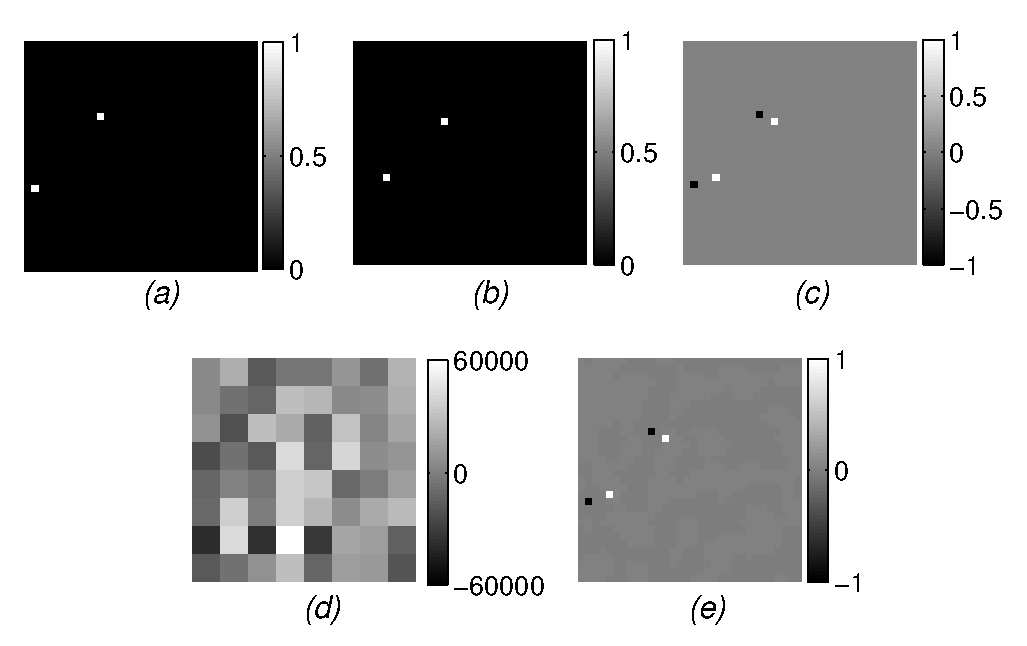
\includegraphics[scale=0.75]{scout_fig10_v2.eps}
	\captionof{figure}[Difference frame 1 of a sequence of two movers on a black background.]{A reconstruction of a $32 \times 32$ scene with two movers of equal amplitude on a black background. (a) ground-truth scene 1 (b) ground-truth scene 2 (c) ground-truth frame difference and (d) measured $8 \times 8$ frame difference, scaled so that it is discernible (e) reconstructed $32 \times 32$ difference frame}
	\label{fig:scout_fig10_un}
\end{figure}

\begin{figure}
	\centering
	\includegraphics[scale=0.75]{scout_fig11_v2.eps}
	\captionof{figure}[Difference frame 9 of a sequence of two movers on a black background.]{A reconstruction of $32 \times 32$ scene with two movers of equal amplitude on a black background. This frame shows the results when the past and present mover locations are adjacent in the difference frame. (a) ground-truth scene 1 (b) ground-truth scene 2 (c) ground-truth frame difference and (d) measured $8 \times 8$ frame difference, scaled so that it is discernible (e) reconstructed $32 \times 32$ difference frame}
	\label{fig:scout_fig11_un}
\end{figure}


\begin{figure}
	\centering
	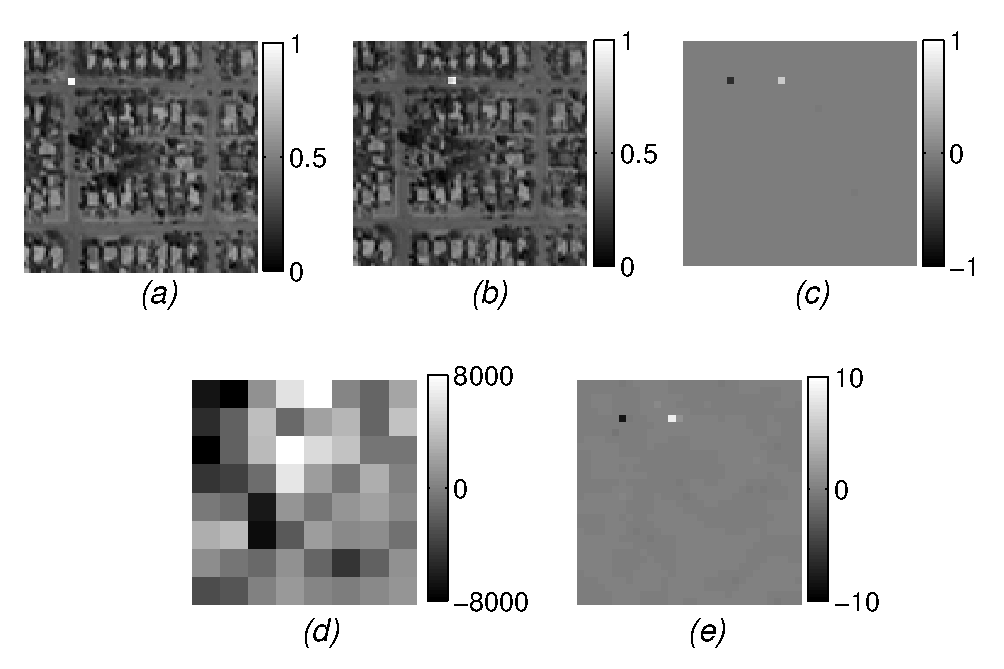
\includegraphics[scale=0.75]{scout_fig12_bg_un}
	\captionof{figure}[Difference frame 1 of a reconstruction video of two movers on a non-zero background.]{Difference frame 1 of a video demonstration of compressive tracking of a  $32 \times 32$ difference scene with a non-zero background. Scene background ©2012 Google. (a) ground- truth scene 1 (b) ground-truth scene 2 (c) ground-truth frame difference and (d) measured $8 \times 8$ frame difference, scaled so that it is discernible (e) reconstructed $32 \times 32$ difference frame}
	\label{fig:scout_fig12_bg_un}
\end{figure}


In the reconstruction of the ninth difference frame, the amplitude of one the movers had a lower amplitude, shown in \Cref{fig:scout_fig11_un}. Poor reconstruction tends to occur when two movers are located adjacent to each other in the ground-truth difference scene. This is an issue that can be traced to the system response matrix $\mb{H}$, locations next to each other have are more likely to have larger correlations in their respective \gls{psf}.


We also performed a more realistic experiment in which a mover simulates a vehicle driving on a street. This demonstrates that the \gls{scout} works well in situations with non-zero backgrounds. This sequence with the results for a single mover is also shown in Appendix \ref{app:scoutExpResults}. The first difference frame of this sequence is shown in \Cref{fig:scout_fig12_bg_un}. As seen in ground truth difference fram $\Delta \mb{f}$ shown in \Cref{fig:scout_fig12_bg_un}(c), the amplitude of the past and present mover locations in the ground-truth are lower than the zero background case. Therefore there is also less contrast in $\Delta \mb{g}$ the difference measurements in \Cref{fig:scout_fig12_bg_un}(d), which makes this case more sensitive to noise. 

The most notable feature in the non-zero background results is less quantitative agreement with the ground-truth, even when the calibration matrix is scaled according to \Cref{eq:ScoutCalibrationMatrixScaling}. There are several reasons for this: Nonlinearities in the overall system response that result from a nonlinear monitor “gamma” (mapping from pixel value to output brightness) and inter-pixel interactions that effect brightness. These effects are not captured during calibration as that is performed point-by-point (thus reducing inter-pixel effects) and with pixels that are fully-on or -off (thus avoiding effects from monitor gamma). Another possible reason is over-multiplexing, since the total light from each frame is increased, there is less dynamic range in the \gls{fpa}, and therefore detector non-linearity may be a source of error. Despite the lack of quantitative agreement, qualitative agreement is excellent and the movers are clearly identifiable agains the background in \Cref{fig:scout_fig12_bg_un}(e).



\section{Conclusion}

While the \gls{scout} architecture is well-suited for tracking applications, it does have limitations which make it less useful for general imaging applications. Without sparse scene motion, the priors used in reconstruction will lead to incorrect results. Reconstructions only show the locations of moving objects, and the sensing platform must be stationary relative to the scene so that frame differences are sparse. However, more sophisticated techniques could potentially estimate platform motion. Despite the limits of the \gls{scout}, the architecture is well-suited for applications such as fixed-camera wide-area surveillance where bandwidth, data volume, and cost are key concerns.

Many of the theoretical guarantees for \gls{compressive sensing} is not specialized or tuned for the block-circulant system matrix. As I mentioned in \Cref{chap:Formalism}, random coding has several theoretical properties that make them useful for compressive sensing. There has been some research work to investigate system matrices with Toeplitz and circulant structure \cite{bajwa2007toeplitz, rauhut2009circulant, romberg2009compressive}, however there has been relatively little work published discussing the approximately block-Toeplitz structure that naturally arises in optical systems such as \gls{scout} and theoretical guarantees like the ones force random coding. Two exceptions are \cite{sebert2008toeplitz, liu2008sparsesense}, which provide both theoretical evidence for the viability of CS system matrices with block-Toeplitz structure.


A completely parallel compressive imager would require as many encoding optical elements as simultaneous measurements. The \gls{scout} architecture eliminates this scaling issue by giving up the ability to implement arbitrary projections. Using a pair of masks at different distances to create a block-circulant system matrix, the system makes compressive measurements and reconstructs frame differences. The system can be optimized by adjusting system parameters such as mask pitch and defocus distance. Simulations demonstrated the use of the a modified coherence parameter as an efficient predictor of system matrix performance to optimize these parameters. An experimental system based on the \gls{scout} architecture successfully performed compressive motion tracking on scenes with zero and nonzero backgrounds in most instances. However, the reconstruction of difference scenes with adjacent mover locations caused issues due to the design or calibration of the system matrix. The system showed promising results using a general $\ell_1$-norm minimization algorithm and we believe that further research on sparse reconstruction with block-circulant system matrices may decrease reconstruction error. We also believe that non-isomorphic calibration techniques and adding further degrees of freedom in the design parameters could result in significant performance gains.





%\chapter{Adaptive Feature Specific Spectral Imaging-Classifier}\label{chap:Afssic}

This chapter introduces the reader the \gls{afssi-c}.


%\bibliographystyle{IEEEtranS}  
%\bibliography{ThesisBib}




%\chapter{Computational Spectral Unmixing}\label{chap:Csu}

\section{Introduction}

In \Cref{chap:Afssic}, I argued that spectral classification is the goal of spectral imaging in most cases. However, in certain situations the analyst is interested in quantifying the presence of several materials in a single spatial location from a \gls{mixed spectrum}. Mixed spectra can occur when the sensor is part of a high-altitude platform such as an unmanned aerial vehicle (UAV) or satellite. The large standoff distances between the ground and the instrument result in large spatial resolutions. For example, in the Hyperion Imaging Spectrometer, which is satellite based, the spatial resolution is 30 meters \cite{folkman2001eo}. One cannot reasonably expect a single material to always occupy that large of an area. \Gls{spectral unmixing} is any procedure which attempts to take the measured spectrum of a mixed pixel and decompose it into a set of constituent spectra called the \glspl{endmember} and a set of corresponding fractions called the \glspl{fractional abundance}. 

Traditional spectral unmixing requires several seperate steps to quantify the fractional abunances. The isomorphic sensor must spatially or spectral scan the object scene, building the spectral datacube piece by piece. At each step, the restricted aperture or wavelength range rejects a significant fraction of the availiable light. A post-processing step is then used to reduce the size of the data to reduce the computational load. Finally an inversion step is used to compute the fractional abundances. Intuitively, the advantages of computational sensing discussed throughout this dissertation should be able to ameliorate some of the design trade-offs in traditional spectral unmixing.

In this chapter, I will talk about my efforts to apply the techniques of computational sensing to directly estimate the \gls{fractional abundance} without the need to reconstruct the spectral datacube. I will introduce a computational spectral imaging architecture called the \gls{lcsi}. I will then provide simulation results that demonstate the advantage of computational spectral unmixing using the \gls{afss} and the \gls{lcsi} over traditional architectures by leveraging the Fellgett and Jacquinot advantage with compressive sensing algorithms which promote sparse solutions. Results from a proof-of-principle experiment demonstrate the promise of computational spectral unmixing. 

\section{The Linear Mixing Model}

There are two main reasons why mixed spectra occur \cite{keshava2002spectral, keshava2003survey}. First, if the spatial resolution of the sensor is low enough, separate materials can jointly occupy the \acrfull{fov} of a single pixel, the resulting spectral measurement is a combination of the constituent spectra, see \Cref{fig:linearAndNonlinearMixing}(a). In this case, one can imagine the object scene as a \emph{checkerboard} mixture: light from the illumination source scatters or reflects from only one of the materials before being observed by the sensor, multiple scattering between materials are ignored. The second reason for mixed pixels occurs when different materials are combined into a homogeneous mixture, see \Cref{fig:linearAndNonlinearMixing}(b). In this case, mixed spectra are not caused by poor spatial resolution, they are inherent to the nature of the scene. For the purposes of this chapter I will focus on the first case, mixed spectra causes by the spatial resolution limitations of the sensor.

\begin{figure}
	\centering
	\includegraphics[scale=0.85]{linearAndNonlinearMixing.pdf}
	\captionof{figure}[Linear versus Non-Linear Mixing]{(a) Illustration of linear mixing where incident solar radiation reflects from a surface and the surface consists of distinct materials. (b) Illustration of nonlinear mixing where incident solar radiation encounters an intimate mixture of materials, reflecting or scattering multiple times before being reflected toward the spectral image sensor.}
	\label{fig:linearAndNonlinearMixing}
\end{figure}

When mixed spectra occur due to the spatial resolution limitation of the instrument, the fractional abundance is linearly proportional to the relative area of each material. This is called the \acrfull{lmm}, where the mixed spectrum can be written as 
%
\begin{equation}
\mb{f} = \sum_{r=1}^{N_{R}} x_r \mb{s}_r + \mb{e} = \mb{S} \mb{x}  + \mb{e}
\end{equation}
%
where $\mb{f}$ is the \gls{mixed spectrum}, $\mb{s}_r$ is the $r^{th}$ endmember spectrum, $\mb{S}$ is a matrix in which the columns are the endmember spectra, $\mb{x}$ is the fractional abundance vector, and $N_{R}$ is the number of endmembers in the endmember library, each spectra has \gls{numspecchan} spectral channels. In the \gls{lmm}, the interactions between distinct endmembers are assumed to be neglible \cite{clark1984reflectance}. 

There are two contraints imposed by the physics of the situation. Intuitively we should expect that the fractional abundance should be equal to or larger than zero. This is the \emph{nonnegativity} constraint:
%
\begin{equation}
	x_r \geq 0.
\end{equation}
%
We should also expect that if energy is conserved, i.e. there is no absorption of light, then the \gls{fractional abundance} should sum to one. This is the \emph{additivty} constraint:
%
\begin{equation}
	\sum_{r = 1}^{N_{R}} x_r = 1
\end{equation}


\subsection{Unmixing in Traditional Spectral Imaging}

In traditional spectral imaging, the spectral datacube is first isomorphically acquired by the instrument before any unmixing step is performed. Often a \gls{dimensionality reduction} step is used to reduce the computational burden of processing the spectral datacube \cite{keshava2002spectral, keshava2003survey}. If the endmembers are unknown, an \gls{endmember determination} step is executed. Finally, the \gls{inversion} step is used to estimate the fractional abundances. 

Notable data reduction algorithms include \acrfull{pca} and \acrfull{mnf}. As described in Chapter 2, \gls{pca} is applied to the measured data and finds the basis which decorrelates the data. In \gls{pca} one typically observes a steadily decreasing signal-to-noise ratio as the principal compenent number increases \cite{green1988transformation}. However, this is not always the case, since it equates variance with information and is based on the assumption that the data structure can be described by a multi-dimensional normal distribution \cite{philpot2015mnf}. In \gls{mnf}, the algorithm attempts to order the components in terms of \gls{snr} which consists of two seperate \gls{pca} rotations and a noise whitening step. \gls{mnf} requires estimation of the noise covariance matrix in addition to the covariance of the data.

%A non-statistical technique for dimensionality reduction is the optical real-time adaptive spectral identification system (ORASIS) \cite{bowles2007optical}, which is a series of steps that identify a subset of representative, or exemplar, pixels that convey the variables in a scene. When a new pixel is collects from the scene, a spectrum is compared to each examplar pixel using this angle metrix. If it is sufficently different then it is added to the set. Then using a modified Gram-Schmidt process, an orthogoal basis is created and a new dimension is added until the every exemplar can be represented well within a certain tolerances \cite{keshava2003survey}. 

The inversion step actually estimates the \gls{fractional abundance}. There are a variety of inversion techniques which actually attempt to estimate the fractional abundance vector. Many are based on minimizing the squared error and attempt to enforce additivity or non-negativity \cite{keshava2003survey, lawson1995solving}. There are various algorithms based on \acrfull{map}, \acrfull{mle}, and clustering which can be used for spectral unmxing. Unfortunately, we cannot explore each inversion technique, however due to their prevalence, I will use least-squares based inversion technique when comparing computational spectral unmixing techniques to tradiational unmixing techniques.

\section{Architecture}

In this research, two seperate architectures are used for spectral unmixing. The first architecture is the \gls{afss}, which is the single pixel version of the \gls{afssi-c} described in depth in \Cref{chap:Afssic}. The second architecture is a \acrfull{lcos} based spectral imager, called the \gls{lcsi}, which allows for an extremely compact instrument, see \Cref{fig:lcsiArchi}. The system provides a programmable spectral filter, which can be independently addressed at each physical pixel of the \gls{slm}. The device consists of an array of micro cells of liquid crystal on a reflecting layer \cite{lazarev2012lcos}. Each layer of liquid crystal can be modeled as a thin retarder plate. Since the birefringent phase retarder is sensitive to wavelength, the \gls{lcos} combined with a polarizing beam splitter or a linear polarizer produces a wavelength dependent transmission pattern, a spectral filter, which modulates the input spectra \cite{yuan2015compressive}.

\begin{figure}
	\includegraphics[scale=1.0]{lcsiArchi.pdf}
	\captionof{figure}[LCOS Based Spectral Imager]{The LCOS Spectral Imager. Light from the intermediate image plane is collimated. A polarizing beam splitter passes p-polarized light and rejects s-polarized light. Upon reflection of the LCOS SLM, the polarization state is changed to some elliptical polarization state. Only the s-polarized portion of the elliptical polarization is reflected toward the upper part where it is imaged onto a scientific camera. The intensity of the light that is passed depends on birefringence created by the programmable LCOS.}
	\label{fig:lcsiArchi}
\end{figure}

%\subsection{How the LCOS Creates Spectral Filters}
% Imagine an incident monochromatic plane wave traveling in the z-direction with a Jones polarization vector 
% \begin{equation}
% \mbh{a} = 
% 	\begin{bmatrix}
%     	a_{x}  \\
%     	a_{y} e^{ i \phi  }  \\
%    \end{bmatrix}
% \end{equation}
% %
% where $\phi$ is the phase differene between the x and y axes \cite{milster2013notes}. The full plane wave for the electric field can be written as

% \begin{equation}
% \mb{E} = A \exp \left[ \mb{k} \cdot \mb{r} - \omega t \right] \mbh{a}
% \end{equation}
% %
% where there leading $A$ is a complex constant that adjusted for amplitude and absolute phase shift.
% %
% \begin{equation}
% 	\mb{k} = k \mbh{k} = k \ap{ \alpha \mbh{x} + \beta \mbh{y} + \gamma \mbh{z} }
% \end{equation}
% %
% is the propagation vector with wavenumber $k = 2\pi /\ \lambda$ and direction cosines $\ap{\alpha, \beta, \gamma}$.

% Transmitting through the polarizing beam splitter only passes horizontally polarized light

% \begin{equation}
% 	\begin{bmatrix}
% 		a_x \\
% 		0 
% 	\end{bmatrix}
% 	=
% 	\begin{bmatrix}
% 		1 & 0 \\
% 		0 & 0
% 	\end{bmatrix}
% 	\begin{bmatrix}
% 		a_x  \\
% 		a_y e^{ i \phi  }
% 	\end{bmatrix}
% 	\label{eq:jonesAfterPBS1}
% \end{equation}

% The \gls{lcos} in our architecture is a phase only reflective type. Liquid crystal is used because it has the ability change birefringence $\Delta n$ when an electric field is applied. Birefringence is defined as 
% %
% \begin{equation}
% 	\Delta n = n_e - n_0
% \end{equation}
% %
% where $n_0$ is the ordinary refractive index and $n_e$ is the extraordinary refractive index \cite{zhang2014fundamentals}. By changing the electric field in the cell the $\Delta n$ is changed. 

% Birefringence is utilized to create retardation plates. These retardation plates serve to change the polarization state of input light. If one aligns the retardation plate so that the x polarized light is incident on the ordinary refractive index and the y polarized light is incident onto the ordinary refractive index then x and y polarizations are phase shifted by
% %
% \begin{equation}
% 	\eta = \frac{2 \pi}{\lambda} \left[ n_e\ap{\lambda} - n_o \ap{\lambda} \right] T
% \end{equation}
% %
% where $T$ is the physical thickness of the plate, where the $ n_e \ap{ \lambda } $ and $ n_o \ap{\lambda} $ are index of refraction of the extraordinary and ordinary waves which are wavelength dependant functions \cite{milster2013notes}. 

%The general Jones matrix for an arbitrary birefringent material as a retardation plate is
%
%\begin{equation}
%	\begin{bmatrix}
%		M_{11} & M_{12} \\
%		M_{21} & M_{22}
% 	\end{bmatrix}
% 	=
% 	\begin{bmatrix}
% 		e^{i \eta/2} \cos^2 \theta + e^{-i \eta/2} \sin^2 \theta & \ap{ e^{i \eta/2} - e^{-i \eta/2} } e^{-i \phi} \cos \theta \sin \theta \\
% 		\ap{ e^{i \eta/2} - e^{-i \eta/2} } e^{i \phi} \cos \theta \sin \theta & e^{i \eta/2} \sin^2 \theta + e^{-i \eta/2} \cos^2 \theta
% 	\end{bmatrix}
% 	\label{eq:arbJonesMatrix}
% \end{equation}
% %
% where the relative phase retardation between the fast and slow axes is given by $\eta = \phi_y - \phi_x$, $\theta$ is the orientation of the fast axis with respect to the x-axis, and $\phi$ is the circularity. Thus after propagating from the LCOS the Jones Vector is written as
% %
% \begin{equation}
% 	\begin{bmatrix}
% 		a_x M_{11} \\
% 		a_x M_{21}
% 	\end{bmatrix}	
% \end{equation}
% %
% finally the vertical polarization (y) is reflected by the polarizing beam splitter towards the camera
% %
% \begin{equation}
% 	\begin{bmatrix}
% 		0 \\
% 		a_x M_{21}
% 	\end{bmatrix}	
% \end{equation}

% Where the intensity is pro



% The phase shift can be used to change the polarization state of the light. For example, when linearly polarized light at 45 degrees goes through a phase shift of $\Delta = \lambda / 2$ the polarized light will rotate to vertical. However, this is a special case and in general the output light will be elliptically polarized. When elliptically polarized light is incident onto a linear polarizer, only linearly polarized light is passed, the intensity of the light passed however depends on the relative amplitude and phase of the x and y polarizations of the incident light \cite{milster2013notes}. 

Unfortunately, a full discussion of polarization is not appropriate for this dissertation. The important point is that for light of a single wavelength, the \gls{lcos} produces polarization which in general is not linearly polarized. Placing a linear polarizer after the light has been reflected from the \gls{lcos} will then force the transmitted light to be linearly polarized but at an intensity that depends on the projection of the output polarization from the LCOS onto the transmission direction of the polarizer. Passing non-monochromatic light to an \gls{lcos} and then a linear polarizer will impart a wavelength dependent intensity. In short, the \gls{slm} provides polarization and wavelength dependent transmission patterns to encoded the spectral datacube \cite{tsai2015spatial}.

\subsection{Forward Model}

The forward model for the \gls{lcsi} is similar to the forward model for the \gls{afssi-c} presented in \Cref{ssec:afssicForwardModel}, except now one does not need to account for the dispersion when imaging from the input plane to the LCOS and from the LCOS to the \gls{fpa} of the camera. I will thus skip the derivation of the forward model and simply present the final equation for the measurement value at pixel $n$ and $l$ from the camera:
%
\begin{align} 
	\Gamma_{nl} &= \sum_{n^\prime l^\prime} \iiint \mbox{rect} \left( \frac{x}{\Delta} - l, \frac{y}{\Delta} - n \right) \mbox{rect} \left( \frac{x}{\Delta} - l^\prime , \frac{y}{\Delta} - n^\prime \right) \notag \\
 	&\qquad \times T_{n^\prime l^\prime} \ap{\lambda} D_0 \left( x, y; \lambda \right) dx \, dy \, d\lambda.
\end{align}
%
Notice that there is no dispersion constraint like the one created in the \gls{afssi-c} or a joint spatial-spectral contraints like in the \gls{cassi}. The \gls{lcos} creates dispersion by the very nature of wavelength dependant birefringence. If one so choose to, one can simply treat each pixel in the image as completely indepdent from neighboring pixels. This greatly simplifies the analysis. 

Similar to the \gls{afssi-c} we can further simplify this by imagining a discrete spectral density, the spectral datacube. The discretized source spectral datacube is $D$, and then the detector signal $\Gamma$ is a result of spectral filter created by the \gls{pbs} and LCOS combination where spectral filter $T$ acting on the pixelated source is
%
%
\begin{equation}
	\Gamma_{n,l} = \sum^{N_{\lambda}-1}_{c = 0} T_{n,l,c} D_{n,l,c} \,
\end{equation}
%
%
which shows the measurement at each pixel being the inner product of the source spectrum and the spectral filter created by the \gls{pbs}-\gls{lcos} combination. In a single spatial location, this reduces to a simple inner product
%
\begin{equation}
	g_m = \mb{h}_m^{T} \mb{f} 
\end{equation}
%
where the subscript $m$ represents the $m^{\text{th}}$ measurement step and $\mb{f}$ the true spectrum at that pixel. For a sequence of measurements this simplies to 
%
\begin{equation}
	\mb{g} = \mb{H} \mb{f}
\end{equation}
%
where the $m^{th}$ row of $\mb{H}$ is $\mb{h}_m^T$ and $\mb{g}$ is an $N_m \times$1 vector, $\mb{f}$ is the ground truth mixed spectrum
%
\begin{equation}
	\mb{f} = \mb{S}\mb{x}
\end{equation}
%
Thus for a sequence of noisy measurements at a single pixel
%
\begin{equation}
	\mb{g} = \mb{H}\mb{S}\mb{x} + \mb{e} = \mb{A}\mb{x} + \mb{e}
\end{equation}\label{eq:csuForwardModel}
%
where $\mb{H}$ is an $N_m \times N_{\lambda}$ matrix, $\mb{S}$ is the endmember library which is an $N_{\lambda} \times N_{R}$ matrix, $\mb{x}$ is the fractional abundance vector which an $N_R \times 1$ vector, $\mb{e}$ is the additive noise which is a $N_m \times 1$ vector. If I define
%
\begin{equation}
	\mb{A} = \mb{H} \mb{S},
\end{equation}
%
One can think of $\mb{H}$ as the sensing matrix and $\mb{S}$ as the representation matrix as discussed in \Cref{sec:compressiveSesing}.


\section{Solving the Inverse Problem}

For this work I chose to use the least-squares estimator (LSE)
%
\begin{equation}
	\mbh{x} = \ap{ \mb{A}^T \mb{A} }^{-1} \mb{A}^T \mb{g}
\end{equation}\label{eq:lseEquationChap5}
%
to demonstrate the advantage provided by multiplexing without using compressive sensing based algorithms. To demonstrate compressive sensing approaches, I will used the built-in MATLAB \texttt{lasso} function which attempts to minimize the $\ell_1$ regularized least-squares objective function 
%
\begin{equation}
	\mbh{x} = \argminA_{\mb{x}} \: \| \mb{Ax} - \mb{g} \|_{2}^{2} + \tau \| \mb{x} \|_1
	\label{eq:l1reglsV2}
\end{equation}
%
in order to find fractional abundances that are sparse. 

In the traditional spectral imager, the fractional abundance is estimated after the spectral datacube is acquired. In our work, the fractional abundance can be estimated after each measurement step. However, since we need a way to compare our results to traditional spectral imaging, we can use the tunable filter architectures for a baseline comparision. The tunable filter acquires a single wavelength over the entire field-of-view and thus allows us to obtain measurements in a time sequential manner. This means that we can use the LSE to get an idea of how a traditional spectral imaging architecture would perform.

As I mentioned earlier, in remote sensing the fractional abundance vector $\mb{x}$ tends to be sparse: the number of endmembers in the library is much larger than number of endmembers that are actually present in the mixed spectrum $N_{R} > \| \mb{x} \|_0$. Therefore, one can invoke the techniques designed for compressive sensing to find solutions that are sparse.

\section{Prior work}


\subsection{Prior Efforts in Computational Spectral Unmixing}

Several researchers have shown promising results in applying compressive sensing to spectral unmixing using a modified single-pixel camera architecture \cite{li2012compressive}. They demonstrated the ability to reconstruct the fractional abundance planes without the need to explicitly reconstruct the spectral datacube. In this approach, the object scene is imaged onto a \gls{dmd} and then a condensor lens focuses the reflected light into a whiskbroom spectrometer. One can think of this architecture as a set of parallel single-pixel cameras each operating at a different spectral channel, with the constraint that each \gls{dmd} must display the same pattern. This architecture does not code the spectral dimension of the spectral datacube. The researchers demonstrated compressive unmixing by minimizing the total variation (TV) of the endmember images while enforcing the nonnegativity constraint. 

In another effort, researchers use the \acrfull{cassi} architecture to perform compressive sensing on the spectral datacube and solve the $\ell_1$-regularized least squares problem (lasso in regression) to promote sparsity in the fractional abundances \cite{monsalve2015spectral}. Due to the nature of the single-disperser \gls{cassi} architecture, the researchers are forced to solve a larger joint-inference problem to preform spectral unmixing. 

\subsection{Prior efforts using LCOS Computational Spectral Imaging}

Several groups have previously demonstrated computational spectroscopy and spectral imaging results using variations of liquid crystal technology. The first instance, in 2012, used a single-pixel liquid crystal device to demonstrate compressive spectroscopy and exhibited a 10$\times$ reduction in the number of measurements compared to a traditional ismorphic spectrometer \cite{august2013compressive}. Shortly after in 2013, a demonstration of a compressive spectral imager using an \gls{lcos} \gls{slm} was published which jointly coded spatial and spectral features \cite{zhu2013coded}. In 2015, an \gls{lcos} based hyperspectral imaging sensor demonstrated blind compressive sensing, using a Bayesian approach to dictionary learning \emph{in situ} \cite{yuan2015compressive}. That same year, a miniture ultraspectral imaging system based on a custom built liquid crystal cell, which applies the same spectral filter to each spatial location, demonstrated the ability to reconstruct gigapixel spectral datacubes with an order of magnitude reduction in measurement steps compared to isomorphic systems \cite{august2016miniature}. However, to my knowledge, no one has ever attempted to perform direct spectral unmixing using an \gls{lcos} based device. 


\section{Design and Selection of Spectral Filters for Unmixing}


\subsection{Adaptive Unmixing Algorithm For the AFSSI-C}\label{sec:unmixingAlgo}


The \acrfull{afss} has the ability to display psuedo-arbitrary spectral filters with the restriction of using binary codes $ \{ -1, +1 \}$ using the \gls{dmd}. In the \gls{afss}, one can emulate a tunable filter spectrometer by measuring one spectral channel at time, i.e. turn on one mirror per measurement step. In this case, the measurement matrix is equal to the identity matrix $\mb{H} = \mb{I}$. Combining the tunable filter approach with the LSE produces what one should expect from a traditional isomorphic spectrometer to conduct spectral unmixing.

We can also use random binary codes to achieve a multiplexed measurement to improve the throughput of each measurement to reduce the unmixing error. The spectrum can then be estimated by processing the measurement with the LSE to demonstrate the performance gained by collecting more light per measurement step. However, estimating the fractional abundance using a compressive sensing based algorithm such as the MATLAB \texttt{lasso} function can produce even better unmixing results by enforcing sparsity. 

As shown in the \gls{afssi-c}, adaptive coding can significantly improve performance compared to multiplexing alone. We developed an algorithm for adaptively creating spectral filters which uses a modified version of \gls{ppca} to create adaptive spectral filters. This algorithm begins with the spectral library which consist of the each endmember spectra $\mb{S}$. Initially, before any measurements are made, the estimated fractional abundance of each endmember is assumed to be the same: 
%
\begin{equation}
	\mbh{a}_{m=0} = 
	\begin{bmatrix}
	\frac{1}{N_R} \\
	\frac{1}{N_R} \\
	\vdots \\
	\frac{1}{N_R}
	\end{bmatrix}
\end{equation}
%
where $N_R$ is the number of endmembers. The subscript denotes the $m^{th}$ measurement step. Before any measurement is made, $m=0$. Then each endmember in the spectral library is weighted by the square of their respective estimated fractional abundance
%
\begin{equation}
	\mb{S}_w = 
	\begin{bmatrix}
		\hat{a}_1^2 \mb{s}_1 & \hat{a}_2^2 \mb{s}_2 & \hdots & \hat{a}_{N_R}^2 \mb{s}_{N_R}
	\end{bmatrix}
	\label{eq:weightedSpectralLibrary}
\end{equation}
%
this is called the weighted spectral library. Then the eigenvectors of the unnormalized covariance matrix of the weighted spectral library are computed to obtain the principal components
%
\begin{equation}
	\mb{X}_m = \mb{S}_w \mb{S}_w^T.
\end{equation}
%
Where the first principal component corresponds to the direction of largest variance and so on. Initially, for the first measurement, the algorithm chooses the first principal component for the spectral filter $\mb{h}_{m=1} = \mb{p}_1$. The measurement is then recorded
%
\begin{equation}
	g_{m=1} = \mb{h}_{m=1}^{T} \mb{f} + e_{m}
\end{equation}
%
A simulated ``guess'' measurement based on the current estimated fractional abundance $\mbh{a}_{m -1}$ is also computed:
% 
\begin{equation}
	\gamma_{m=1} = \mb{h}_{m=1}^{T} \mb{S} \mbh{a}_{m=0}
\end{equation}
%
notice that the guess measurement does not include any simulated noise. Remember $\mb{S}$ denotes the original spectral library matrix, not the weighted spectral library matrix. After the measurement is recorded, the $\ell_2$ norm of the difference between the guess measurement and the actual measurement is recorded:
%
\begin{equation}
	\xi_m = \| \gamma_m - g_m \|_2 
\end{equation}
%
The fractional abundance is then estimated using the MATLAB \texttt{lasso} function. In practice, the LSE is used for the first measurement step since the function \texttt{lasso} requires atleast two rows for $\mb{A}$ and therefore two measurements, to run. 

The spectral library is then reweighted using \Cref{eq:weightedSpectralLibrary}. Again the principal components are recomputed. For the $m^{th}$ measurement step, the $m^{th}$ principal component is used for the spectral filter. After the measurement has been recorded, the  $\ell_2$ norm of the difference between the guess measurement and the actual measurement is recomputed $\xi_m$. 

%Again the weighted spectral library is recomputed as well as the principal components. 

This continues after each measurement until either two things happen: 
\begin{enumerate}
	\item If the current $\ell_2$ norm of the difference between the guess and the actual measurement exceeds the last $\ell_2$ norm of the difference between guess and actual measurement by
	%
	\begin{equation}
		\xi_m > \xi_{m-1} - \frac{\sigma}{2}
	\end{equation}	
	%
	where $\sigma$ is the standard deviation of the system noise, which is assumed to be \gls{awgn}.

	\item Used the sixth principal component.
\end{enumerate}

when either of these two conditions are met, the loop resets to using the first principal component again. I constrained the algorithm to only use the first six principal components, because I noticed that the unmixing preformance is optimized when limited to only the first six principal components. Intuitively, this may be occuring because higher principal components tend exhibit lower SNR or because the spectra in the library do not exhibit significant high frequency features. This algorithm is called \acrfull{swpca}. It is important to note that as of yet, this algorithm does not consider the dispersion constraint of the \gls{afssi-c}, and therefore is more appropriate for the single pixel version, the \gls{afss}. The MATLAB code which simulates \gls{swpca} is found in Appendix \ref{app:adaptiveUnmixAlgo}.


\subsection{Hybrid Spectral Filters for the LCSI}\label{ssec:hybridFiltersLCSI}

The spectral filters produced by the \gls{lcsi} architecture are constrained by the physics of the birefringence dispersion created by the \gls{lcos}. For our particular model, the Holoeye PLUTO LCOS SLM, the spectral filter is changed by sending a different grayscale value to the green channel of the video input (Holoeye allows their SLM to be connected like a second monitor). Since there are 256 grayscale values (0-255), there are 256 different spectral filters, see \Cref{fig:slmSpectralFiltersVisible}. 

Since one is not able to design the spectral filters individually, the next best thing is to choose which spectral filters should be used at each measurement step. Intuitively, one can imagine that using the same spectral filter over and over again will lead to a measurement matrix $\mb{H}$ where the rows are linearly dependent. Instead, one should strive to construct a measurement that is highly incoherent to satisfy the \acrfull{rip}. 

For my experiment, I will compare several methods of choosing the spectral filters. The first method is simply selecting them at random from a discrete uniform distribution between 1 and 256, while constraining the selections to prevent using the same spectral filter from being used more than once. This technique however does not attempt to incorporate any prior knowledge about the statistics of the endmembers, besides sparsity. 

One attempt to incorporate the statistics of the endmembers is to use \gls{pca} to select the spectral filters. One could imagine an algorithm which computes the principal components of the endmembers (spectral library) and then selects the spectral filters which most closely resemble the principal component vector $\mb{p}$ based on their angle:
%
\begin{equation}
	\mb{h} = \argmaxA_{\mb{h}} \: \left\{ \frac{ \mb{p} }{ \| \mb{p} \| } \cdot \frac{ \mb{h} }{ \| \mb{h} \|  } \right\}.
\end{equation}
%
For the $m^{th}$ measurement, the spectral filter whose dot product is largest with the $m^{th}$ principal component of the endmember matrix is selected. However, using all the principal components actually increases the unmixing error after a certain amount of measurement steps, as compared to purely random selections. This occurs for several reasons: As the PC number increases, they actually become less informative. Second, principal components tend become more rapidly varying as the PC number increases, the spectral filters generated by the LCOS are in general smoothly varying and become more difficult to match with the higher principal components.

Thus, we created a hybrid spectral filter selection technique that uses \gls{pca} to select the first several spectral filters and then uses psuedo-random selections after a certain number of measurement steps. This balances the ability of \gls{pca} to choose spectral filters that improve the unmixing error at the initial measurement steps while using random selections to ensure the measurement matrix is incoherent enough to satisfy the \gls{rip}.

The hybrid approach to selecting the spectral filters is further extended to use a more advanced version of \gls{pca} called \acrfull{mnf} transform. \gls{mnf} was originally developed to remove noise from multispectral satellite images \cite{green1988transformation} and attempts to select a basis which orders the signal-to-noise ratio of the MNF components. However, \gls{mnf} is also used for Blind Signal Seperation (BSS), which is the seperation of a set of source signals from a set of mixed signals \cite{hundley2001solution}. Instead of computing the principal components, I compute the maximum noise fraction components of the spectral library. I specifically used the noise adjusted principle component analysis (NAPCA) algorithm to compute the MNF of the spectra library which is found in \cite{hundley2001solution}. The algorithm associates rapidly varying parts of the spectral library with noise and assumes the signal is contained in the smoothly varying parts of the spectral library. 

\begin{figure}[H]
	\centering
	\includegraphics[scale=0.75]{slmSpectralFiltersVisible.pdf}
	\captionof{figure}[The normalized spectral filters created by the Holoeye PLUTO SLM and polarizing beam splitter]{The spectral filters created by the Holoeye PLUTO SLM and polarizing beam splitter. Each column is a spectral filter at a particular grayscale level (0-255) sent to the PLUTO SLM by a custom MATLAB program. }
	\label{fig:slmSpectralFiltersVisible}
\end{figure}


\section{Results}

\subsection{Simulation Results For the AFSS}

Now that I have discussed various coding strategies for spectral unmixing using the \gls{afss}, it is important quantify  them. I performed simulations over five \gls{snr} levels from $10^{-2}$ to $10^2$, where the \gls{snr} is defined as 
%
\begin{equation}
	\text{SNR} = \frac{ \text{E} \Big[ \text{Var}_{N_{\lambda}  \ap{ \mb{s} } } \Big] }{\sigma^2},
\end{equation}
%
which is the ratio of the average variance of the endmembers over the spectral channels to the noise variance. The results after 40 measurement steps are shown in \Cref{fig:unmixingTechniquesComparison}, which show the average \acrfull{rmse} of the estimated fractional abundance versus SNR. \gls{rmse} is defined as 
%
\begin{equation}
	\text{RMSE} =  \left[ \frac{1}{N_R} \sum_{r = 1}^{N_{R}} \ap{ \hat{a}_r - a_r }^2 \right]^{\frac{1}{2}}
\end{equation}
%
The purple dotted line represents the performance of a tunable filter architecture combined with the least-squares estimator (LSE). With random binary patterns, one can obtain an improvement of approximately 3$\times$ which demonstrates the advantage of multiplexing, as shown in the mustard dash-dotted line. By incorporating the prior knowledge of sparsity of the fractional abundance a futher improvement is also achieved, as shown in the orange dashed line. Finally, the blue solid line represents how adaptively designing the spectral filters and using compressive sensing provides an even better result than random coding alone. 

\Cref{fig:unmixingVsMeasurement} shows the average RMSE as a function of measurement number for SNR = 0.01, 1, and 100. The blue line represents psuedo-random spectral filters, the error decreases monotonically with measurement number as one would expect. The green lines represent what happens if the adaptive algorithm never went back to the first principal component once either of the two conditions in \Cref{sec:unmixingAlgo} are met. Simply using higher principle components does not reduce the RMSE after a certain point, even when the spectral library is weighted by the fractional abundance. The red line represents the adaptive algorithm as discussed. This demonstrates the importance of going back to the first principal component whenever the two conditions are met in the adaptive algorithm: it breaks the performance plateau and significantly reduces the unmixing error compared to random coding alone.

\begin{figure}
	\centering
	\includegraphics[scale=0.70]{unmixingTechniquesComparison.pdf}
	\captionof{figure}[Comparison of Spectral Unmixing Techniques for the AFSSI-C at five different SNR levels]{A comparison of spectral unmixing techniques for the AFSSI-C at five different SNR levels. The y-axis represents the average RMSE of the estimate fractional abundance. The x-axis represents the signal-to-noise in the measurements. The tunable filter LSE refers to the average unmixing performance if one were to use a tunable filter spectral imaging architectures with least squares estimation to estimate the fractional abundance. The random LSE line refers to the improvement in spectral unmixing This shows the improvement that multiplexing provides over simple tunable filter spectral imaging using the least squares estimator (LSE). Then using the multiplex advantage and algorithms that promote sparsity when the fractional abundance is known to be sparse, one can significantly outperform }
	\label{fig:unmixingTechniquesComparison}
\end{figure}

\begin{figure}
	\centering
	\includegraphics[scale=0.70]{unmixingVsMeasurement.pdf}
	\captionof{figure}[Comparison of Spectral Unmixing Techniques for the AFSSI-C versus Measurement Duration]{Comparison of Spectral Unmixing Techniques for the AFSSI-C versus Measurement Duration for SNR = 0.01, 1.0, and 100. Even though the spectral library is weighted by the fractional abundances from the last measurement, simply using every principal component underperforms using random spectral filters with $\ell_1$ regularized least squares (lasso). Switching the principal components according the algorithm described in \Cref{sec:unmixingAlgo} siginificantly reduces the unmixing error. }
	\label{fig:unmixingVsMeasurement}
\end{figure}


\subsection{Initial Experimental Results of Compressive Unmixing Using the AFSSI-C}

I performed an initial proof-of-principle experiment using the \gls{afssi-c} architecture. Due to the dispersion contrainst of the AFSSI-C, I was unable to test the adaptive algorithm, however the random coding and the use of sparsity promotting algorithms can still be demonstrated. 


For this experiment I had to upgrade the \gls{afssi-c} prototype by adding a second display, see \Cref{fig:unmixingArch1}. This is because the original prototype used only one LED computer monitor, so it can only display combinations of the same red, green, and blue (RGB) spectra, producing only three endmembers. In order to have six endmembers, I added an OLED display which also has red, green, and blue spectra but are different enough that they are not simply scaled versions of the RGB spectra from the LED monitor. This is shown in \Cref{fig:unmixingLibrary}. Note that the RGB spectra from the LED look different from \Cref{fig:afssicSpecLib} which was used for the \gls{afssi-c} experiment because the transmission from the pelicle beam splitter also acts as a spectral filter. 

\begin{figure}
	\centering
	\includegraphics[scale=0.70]{unmixingLibrary}
	\captionof{figure}[Six Endmember Spectra Used For Spectral Unmixing Experiment]{The six endmember spectra used for the spectral unmixing experiment. The library consist of the red, green, and blue spectra from an LED Monitor and the red, green, and blue spectra from the OLED. The LED monitor spectra may look different from the one shown in Chapter 4 since the spectra have been modified by transmitting through a pellicle beam splitter. }
	\label{fig:unmixingLibrary}
\end{figure}

\begin{figure}
	\centering
	\includegraphics[scale=1.00]{unmixingArch1.pdf}
	\captionof{figure}[Unmixing Architecture for Spectral Unmixing Experiment]{Experimental architecture used to superimpose the spectral images from the LED monitor, which already was in place, and an OLED display. ZEMAX was used to find the correct location of the achromatic doublet, OLED display, and pellicle beam splitter to ensure the intermediate image from both displays appeared at the same location and with the same transverse magnification.}
	\label{fig:unmixingArch1}
\end{figure}

The first-order optical architecture of the unmixing setup was carefully determined using a ray tracing and optimization software package called Zemax. The goal was to ensure that the intermediate image of the LED monitor and the intermediate image of the OLED were at the same location with the same image size. The two images effectively creates a single image which has spectrally mixed pixels with six possible endmembers. The pellicle beam splitter has a clear aperture of 2 inches, thus it needed to be close enough to the objective lens to minimize vignetting. A commercial off-the-shelf 120 mm EFL achromatic doublet from Edmund optics was placed between the OLED and the pellicle beam splitter to move the OLED closer to the instrument. Once all the optical components were optimized in Zemax, they were exported to Solidworks, see \Cref{fig:solidworksOfMixingSetupPicture}, where mounts for the achromatic doublet and the OLED display were designed for 3-D printing. 

There were several practical experimental issues that had to be addressed. Once the setup was constructed, I used a similar spectral calibration procedure from the \gls{afssi-c} experiment to determine the endmembers from the OLED display. The spatial calibration procedure was identical. The OLED was much brighter than the LED monitor, when measured by the SBIG camera. Second, even though the setup was optimized in Zemax, the actual alignment was imperfect. This caused the right side of the OLED to have a larger point-spread function than the left side of the monitor, which caused spatial cross-talk between neighboring pixels. To compensate for this, only one-fourth of the physical pixels were used in a single system pixel. Then a neutral density filter was placed front of the OLED to make the system pixel intensity on the same order-of-magnitude as the intensity from a system pixel from the monitor. Since the pellicle beam splitter acts as a partially reflecting mirror for OLED, I had to account for the image flip by writing a custom MATLAB function which accounts for the left-right flip. 

\begin{figure}
	\centering
	\includegraphics[scale=0.75]{solidworksOfMixingSetupPicture.png}
	\captionof{figure}[Computer Aided Design (CAD) drawing of experimental mixing setup.]{Computer Aided Design (CAD) drawing of experimental mixing setup. Various objects have been ``hidden'' to reduce clutter and emphasize the essential objects: the OLED, the custom design mount for the OLED, the achromatic doublet and the custom designed mount for the doublet, the pellicle beam splitter shown in a kinematic mount, the objective lens also in a custom fabricated C-mount lens.}
	\label{fig:solidworksOfMixingSetupPicture} 
\end{figure}

In order to perform an experiment which demonstrates the ability of the \gls{afssi-c} to perform unmixing on spectrally mixed images, I displayed a 32 $\times$ 32 green ramp on the monitor, see \Cref{fig:linearGreenRampImages}(a). The intensity of the green increases from left to right. The opposite image is displayed on the OLED display, see \Cref{fig:linearGreenRampImages}(b), the intensity of the green decreases from left to right. The other four endmembers which consists of the red and blue of each monitor are set to zero. The fractional abundance of green from both displays sum to one over the entire region-of-interest. 


\begin{figure}
	\centering
	\includegraphics[scale=0.75]{linearGreenRampImages.pdf}
	\captionof{figure}[Ground Truth Images for Spectral Unmixing Experiement]{Ground Truth Images for Spectral Unmixing Experiement. (a) A linear green ramp on the monitor. (b) A linear green ramp on the OLED. Remember that the green of each display are different.}
	\label{fig:linearGreenRampImages} 
\end{figure}

At each measurement step, the DMD is commanded to display a binary random pattern. Since the pattern is designed for $\{ -1, +1 \}$ values, I had to display the positive pattern, record the camera measurement, then display the negative pattern, and record another camera measurement, then subtract the negative from the positive camera images. This unfortunately introduces an additional factor of $\sqrt{\sigma}$ of measurement noise into each measurement step. Both the LSE and the MATLAB \texttt{lasso} function are used to estimate the fractional abundance. \Cref{fig:rmseVsMeasurementExperiment} shows the average RMSE versus measurement number over the 32 $\times$ 32 region. Unfortunately, due to time constraints, I was unable to develop a procedure to estimate the noise in the experiment, therefore the results cannot be directly compared to the simulation results. The result after the $40^{th}$ measurement is shown in \Cref{fig:linearGreenRampImagesExpResultMeas40} 

 By looking at an example pixel, see \Cref{fig:unmixingResultLinearGreenRamp3232}, one can see that the experiment properly identified the two endmembers that were actually present out of the six total endmembers and was able to accurately estimate the fractional abundance after five measurements. 


\begin{figure}[H]
	\centering
	\includegraphics[scale=0.65]{rmseVsMeasurementExperiment.pdf}
	\captionof{figure}[Average RMSE of 32 $\times$ 32 Experimental Spectral Unmixing Results Using the AFSSI-C]{32 $\times$ 32 Experimental Spectral Unmixing Results Using the AFSSI-C with random binary spectral filters. The MATLAB \texttt{lasso} function outperforms the least squares estimator as the number of measurements increase. Thus have an opportunity to beat traditional systems using significantly fewer measurements}
	\label{fig:rmseVsMeasurementExperiment} 
\end{figure}

\begin{figure}[H]
	\centering
	\includegraphics[scale=0.65]{linearGreenRampImagesExpResultMeas40.pdf}
	\captionof{figure}[Image of 32 $\times$ 32 Experimental Spectral Unmixing Results Using the AFSSI-C after the $40^{th}$ measurement.]{Image of 32 $\times$ 32 Experimental Compressive Spectral Unmixing Results Using the AFSSI-C after the $40^{th}$ measurement.}
	\label{fig:linearGreenRampImagesExpResultMeas40} 
\end{figure}

\begin{figure}[H]
	\centering
	\includegraphics[scale=0.65]{unmixingResultLinearGreenRamp3232.pdf}
	\captionof{figure}[Single Pixel Experimental Spectral Unmixing Results Using the AFSSI-C]{Single Pixel Spectral Unmixing Results with the AFSSI-C with random binary spectral filters. The MATLAB \texttt{lasso} function correctly identifies fractional abundance of the two green spectra from each display within five measurement steps. The four other spectra are estimated to be zero. }
	\label{fig:unmixingResultLinearGreenRamp3232} 
\end{figure}


\subsection{Simulation Results For the LCSI}

In order to accurately simulate the spectral filters I first performed a calibration procedure to measure how the each grayscale level filters an input spectrum. A high intensity custom-built white LED lamp was used to illuminate the \gls{lcsi}. At the output we placed an Ocean Optics USB 4000 spectrometer. Then the spectrum of the white light filtered by \gls{lcsi} at each grayscale level is recorded. Then the spectrum at each grayscale level is normalized by the maximum intensity at each wavelength which produces the calibration spectral filters shown in \Cref{fig:slmSpectralFiltersVisible}.

 In order to quantify the filter selection techniques discussed in \Cref{ssec:hybridFiltersLCSI}, I also produced several simulations. simulated the filter selection technique for SNR = 100. \Cref{fig:lcsiResults1} demonstrates the three techniques: randomly selecting filters, the hybrid PCA-Random filter selection, and the hybrid MNF-Random filter selection. Randomly selecting the filters adequately reduces the unmixing error monotonically with measurement error as expected. By using PCA to select the first six spectral filters the and then using a psuedo-random filter selection technique for the rest a significant performance gain is obtained wthin the first 20 measurements. As the number of measurement numbers increases, the probability of having used all the same spectral filters increases. At measurement 256, when all the spectral filters have been used, the average RMSE is the same. Using a hybrid MNF-Random filter selection produces an additional reduction in unmixing error.


\begin{figure}[H]
	\centering
	\includegraphics[scale=0.70]{lcsiResults1.pdf}
	\captionof{figure}[Comparing Random and Hybrid Spectral Filter Selections for the LCSI]{Comparing Random and Hybrid Spectral Filter Selections for the \gls{lcsi} at SNR = 100. One cannot generate arbitrary spectral filters with the \gls{lcsi}, therefore one must decide how to select from a set of 255 possible spectral filters. A hybrid of using the spectral filters that are closest in angle to the first six principal components and then using random filter selections outperforms purely random filter selections. Similarly, a hybrid of using the spectral filters that are closest in angle to the \gls{mnf} components for the first six measurement steps and then using random filter selections outperforms the random and the PCA-random hybrid filter selection. }
	\label{fig:lcsiResults1}
\end{figure}

\section{Conclusion}

Computational spectral unmixing is a computational sensing approach to estimating the fractional abundances of mixed spectra without the need to directly reconstruct the hyperspectral datacube. I discussed two separate architectures for spectral unmixing, the \gls{dmd} based \gls{afss} and the \gls{lcos} bases \gls{lcsi}. I developed two seperate approaches for coding the mixed spectral measurements for a compressing sensing approach for unmixing. The first used adaptive spectral filters combined with conditions to prevent the unmixing error from plateauing. The second relies on variation of \acrfull{pca} or \acrfull{mnf} to find spectral filters provide very informative measurements compared to simplying selecting spectral filters at random. Simulations show the viability these techniques to significantly reduce the unmixing error over naively random coding (or filter selection) alone, demonstrating the importance of incorporation the prior knowledge of the statistics of the signal-of-interest. 
%\chapter{Conclusion}\label{chap:Conclusion}

This dissertation discussed several important practical considerations of computational sensing and how they are addressed in three separate applications: compressive object tracking, adaptive spectral image classification, and compressive spectral unmixing. As computational sensing continues to make rapid progress in the coming years many of these issues must be addressed and confronted. 

The first chapter introduced the reader to the concepts of isomorphic and computational sensing. Computational sensing was developed from the disparate fields of multiplexing spectroscopy and indirect imaging. However, the development of the \gls{ccd}, the digital computer, and data compression allowed scientists to begin creating practical and reliable demonstrations of computational sensing. The advent of the mathematics and algorithms of compressive sensing generated an additional technological leap which dramatically reduced the number of measurements in order to reconstruct the signal of interest. Once the history and benefits of computational sensing was discussed, I then discussed the practical issues of computational sensors: calibration, over multiplexing due to finite dynamic range and quantization resolution, code design and optimization, and the need for a priori knowledge.

The second chapter formally developed the concepts related to computational sensing. I discussed the Fellgett advantage, using Hadamard and S-matrix multiplexing. Then a formal discussion of \acrfull{pca} was developed, which demonstrates how it can be used as a dimensionality reduction technique which creates a basis that decorrelates the data. Then a formal discussion on Bayesian statistics was given which justified their use in the \gls{afssi-c}. Sparsity, incoherence, and the \acrfull{rip} were discussed in-depth to demonstrate why random coding is popular for acquiring sparse signals in compressive sensing. The $\ell_1$ minimization subject to data agreement constraints and its equivalent problem minimizing the $\ell_1$ regularized least squares objective function were also discussed with some intuition as to why it works well for promoting sparse solutions to undetermined inverse problems. 

The \acrfull{scout} was discussed in the third chapter. The \gls{scout} showed how intentionally blurring the \acrfull{psf} in a compressive imager can actually help reduce the effects of overmultiplexing. As the amount of signals being sensed increases the variations in the sensed single become more difficult to discern. Overmultiplexing occurs due to the finite dynamic range and quantization resolution. In the single pixel camera \cite{duarte2008single}, one is forced to measure a series of projections in a time sequential manner prior to solving an inverse problem, in the \gls{scout} the projections occur in parallel for a single difference scene. The \gls{scout} introduced the reader to the importance of calibration in a compressive sensor. The measurement matrix must be carefully measured to produce optimal results. It also demonstrated that optimizing the measurement matrix can be extremely time consuming by hand. Developing a heuristic method based on the coherence metric and ray based simulations reduced the time it took to find optimal design parameters. 

The fourth chapter discussed the \acrfull{afssi-c} which is a computational spectral image sensor designed to adaptively classify spectra at each location in the field-of-view of the sensor. It used back-to-back spectrographs with a digital micro-mirror device (DMD) to produces psuedo-arbitrary spectral filters at each system pixel. After each measurement, an algorithm updates the probabilities of each spectra and weighted the spectral library before recomputing principal components. The first principal component vector is then used as the spectral filter for each measurement. The \gls{afssi-c} is shown to quickly converge to the correct spectrum significantly outperforming traditional spectral imaging architectures especially in low \gls{tsnr} scenarios. The chapter discussed the development of spatial and spectral calibration procedures, vital for optimal performance of the \gls{afssi-c}. A procedure for estimating the system noise was also described in-depth. 

The fifth chapter discussed an extension of spectral classification called spectral unmixing. Two architectures were discussed for spectral unmixing: the \acrfull{afss} and the \acrfull{lcsi}. The \gls{lcsi} relies on the wavelength dependent nature of birefringence to generate multiplex spectral measurements. One of the major constraints of the \gls{lcsi} is that psuedo-arbitrary spectral filters are not possible like in the \gls{afss} or \gls{afssi-c}, therefore I had to develop techniques for selecting spectral filters using random selections and a hybrid of using \gls{pca} or \gls{mnf} to select spectral filters and then using the random filter selections. 

\section{Future Outlook}


One research project that has been an active area of research in the \acrfull{LENS} is the coded memory effect imaging system being developed by my colleague Xiaohan Li. The project combines the memory effect of speckle with \acrfull{cacti} to temporally code speckle. This allows one to infer dynamic object information that is not directly observable with the speckle alone. 

Computational sensing continues to have an extremely promising future. Large companies are actively conducting research and developing products which take advantage of the principles of computational sensing. For example, Microsoft sells a depth sensor, called the Kinect, which relies on a form computational sensing to infer the distance of objects and their shapes. Meanwhile, a recently announced grant from NASA will fund the development of snapshot hyperspectral imagers based on the \acrfull{ctis} for space-borne applications \cite{ricespectraleyes2016grant}. Many university based research groups around the world are actively conducting research that demonstrate compact spatial, spectral, temporal, and polarization computational sensing. Computational sensing will become even more prevalent as the demand for higher resolutions in resource constrained environments abound. 
%\bibliographystyle{IEEEtranS}  
%\bibliography{ThesisBib}





\renewcommand{\baselinestretch}{1}		% chaning the value
\small\normalsize						% switch size to make the value take

%\printglossaries[type=acryonym]
\printglossaries


\bibliographystyle{IEEEtran.bst}
\bibliography{Dissertation}

\end{document}

